%   Based on the frontespizio (title page) template by Marco Antonio Corallo.

% Document type: the twoside setting makes chapters begin with their first page on the right. 
\documentclass[a4paper, twoside,openright]{report}

% Page margins options
\usepackage[a4paper,top=3cm,bottom=3cm,left=3cm,right=3cm]{geometry} 
% removes this restriction by allowing font sizes at arbitrary sizes
\usepackage{lmodern}
% font size
\usepackage[fontsize=13pt]{scrextend}
% Language(s) of the document contents
\usepackage[english]{babel} % ,italian
% Bibliography language
\usepackage[fixlanguage]{babelbib}

% Bibliography package
%Includes "References" in the table of contents
\usepackage[nottoc]{tocbibind}
% Bibliography package natbib, to have the "author-year" format for citations
\usepackage[round]{natbib} 
% \usepackage{biblatex}

% text encoding
\usepackage[utf8]{inputenc} 
\usepackage[T1]{fontenc}

% For rotating images
\usepackage{rotating}
% To change the header of pages
\usepackage{fancyhdr}               

% Math libraries
% \usepackage{amssymb}
\usepackage{amsmath}
\usepackage{amsthm}         

% For images
\usepackage{graphicx}

% For colors
\usepackage[dvipsnames]{xcolor}        
\definecolor{codegreen}{rgb}{0,0.6,0}
\definecolor{codegray}{rgb}{0.5,0.5,0.5}
\definecolor{codepurple}{rgb}{0.58,0,0.82}
\definecolor{backcolour}{rgb}{0.95,0.95,0.92}
 
% to display programming code
\usepackage{listings}          
\lstdefinestyle{mystyle}{
	backgroundcolor=\color{backcolour},   
	commentstyle=\color{codegreen},
	keywordstyle=\color{magenta},
	numberstyle=\tiny\color{codegray},
	stringstyle=\color{codepurple},
	basicstyle=\ttfamily\footnotesize,
	breakatwhitespace=false,         
	breaklines=true,                 
	captionpos=b,                    
	keepspaces=true,                 
	numbers=left,                    
	numbersep=5pt,                  
	showspaces=false,                
	showstringspaces=false,
	showtabs=false,                  
	tabsize=2
}
\lstset{style=mystyle}

% To insert hyperlinks 

% for referencing images and other labels across documents
\usepackage{xr-hyper}

\usepackage[pdftex,
pdfauthor={Mauro Madeddu},
pdftitle={Assessing Island Effects in Italian Transformer-based Language Models},
pdfsubject={Natural Language Processing},
pdfkeywords={NLP IslandEffects},
pdfcreator={TexStudio}]{hyperref} 

% \externaldocument{chapters/AppendixA}
% \begin{reusefigure}[<float spec>]{<ref>}
	\newenvironment{reusefigure}[2][htbp]
	{\addtocounter{figure}{-1}%
		\renewcommand{\theHfigure}{dupe-fig}% If you're using hyperref
		\renewcommand{\thefigure}{\ref{#2}}% Figure counter is \ref
		%\renewcommand{\thefigure}{\ref{#2} (repeated)}% Figure counter + "(repeated)"
		\renewcommand{\addcontentsline}[3]{}% Avoid placing figure in LoF
		\begin{figure}[#1]}
		{\end{figure}}
	
% For different types of underlinings
\usepackage[normalem]{ulem}

% \usepackage[superscript,biblabel]{cite}

% for tables, allows merging cells across multiple rows
\usepackage{multirow}
\usepackage{array}
\newcolumntype{L}{>{\centering\arraybackslash}m{1cm}}
\usepackage{booktabs}
\usepackage{siunitx}

% for multiple images in a figure
\usepackage{subcaption}

% for numbered lists:
\usepackage{enumitem}

% \usepackage{fullpage}
% \usepackage{amsmath,amssymb,amsthm}

% for image positioning
\usepackage{float}

% for numbering linguistic examples
\usepackage{refcount}
\usepackage{xstring}
% \newcommand{\subref}[1]{\StrRight{\getrefnumber{#1}}{1}} already defined
\usepackage{gb4e} % problem, conflict with other packages
\noautomath

% -----------------------------------------------------------------

% Changes the header style
\pagestyle{fancy}
\fancyhf{}
\lhead{\rightmark}
\rhead{\textbf{\thepage}}
\fancyfoot{}
\setlength{\headheight}{12.5pt}

% Removed the page number on the first page of a chapter
\fancypagestyle{plain}{
  \fancyfoot{}
  \fancyhead{}
  \renewcommand{\headrulewidth}{0pt}
}

% Syntax highlighting for programming code examples
\lstdefinestyle{codeStyle}{
    % Colore dei commenti
    commentstyle=\color{teal},
    % Colore delle keyword
    keywordstyle=\color{Magenta},
    % Stile dei numeri di riga
    numberstyle=\tiny\color{gray},
    % Colore delle stringhe
    stringstyle=\color{violet},
    % Dimensione e stile del testo
    basicstyle=\ttfamily\footnotesize,
    % newline solo ai whitespaces
    breakatwhitespace=false,     
    % newline si/no
    breaklines=true,                 
    % Posizione della caption, top/bottom 
    captionpos=b,                    
    % Mantiene gli spazi nel codice, utile per l'indentazione
    keepspaces=true,                 
    % Dove visualizzare i numeri di linea
    numbers=left,                    
    % Distanza tra i numeri di linea
    numbersep=5pt,                  
    % Mostra gli spazi bianchi o meno
    showspaces=false,                
    % Mostra gli spazi bianchi nelle stringhe
    showstringspaces=false,
    % Mostra i tab
    showtabs=false,
    % Dimensione dei tab
    tabsize=2
} \lstset{style=codeStyle}

% Stile di codice per dimensioni maggiori, in cui ho avuto bisogno di un testo più picolo (ad esempio se si vuole inserire del codice che ha linee molto lunghe). Per usare questo stile piuttosto che il precedente, usare 

% \lstset{style=longBlock}
%  % inserire il codice...
% \lstset{style=codeStyle}

% Il secondo comando consente di tornare allo stile precedente 
\lstdefinestyle{longBlock}{
    commentstyle=\color{teal},
    keywordstyle=\color{Magenta},
    numberstyle=\tiny\color{gray},
    stringstyle=\color{violet},
    basicstyle=\ttfamily\scriptsize,
    breakatwhitespace=false,         
    breaklines=true,                 
    captionpos=b,                    
    keepspaces=true,                 
    numbers=left,                    
    numbersep=5pt,                  
    showspaces=false,                
    showstringspaces=false,
    showtabs=false,                  
    tabsize=2
} \lstset{style=codeStyle}

% si inseriscono nella bibliografia anche le fonti presenti in Bibliography.bib ma non citati direttamente con il comando \cite
\nocite{*}

% Margini prima e dopo blocchi di codice, per avere più distanza
\lstset{aboveskip=20pt,belowskip=20pt}

% Modifica dello stile dei riferimenti, con il testo in cyano
\hypersetup{
    colorlinks,
    linkcolor=Blue,
    citecolor=Blue, % CornflowerBlue, % 
}

% Aggiunti definizioni, teoremi, linea e listing
\newtheorem{definition}{Definizione}[section]
\newtheorem{theorem}{Teorema}[section]
\providecommand*\definitionautorefname{Definizione}
\providecommand*\theoremautorefname{Teorema}
\providecommand*{\listingautorefname}{Listing}
\providecommand*\lstnumberautorefname{Linea}

\raggedbottom

%\newcommand{\cgs}[1]{{\textcolor{brown}[\textcolor{red}{\bf{GS: }}{ \textcolor{brown}{#1]}}}}             
%\newcommand{\cmc}[1]{{\textcolor{blue}[\textcolor{magenta}{\bf{MC: }}{ \textcolor{blue}{#1]}}}}

% for numbered formulas or examples
\theoremstyle{definition}
\newtheorem{thm}{Theorem}[section]
\newtheorem{example}[thm]{Example}


% -----------------------------------------------------------------

\begin{document}

\begin{titlepage}
\begin{figure}[!htb]
    \centering
    
\includegraphics[keepaspectratio=true,scale=0.5]{images/Frontespizio/cherubinFrontespizio.eps}
\end{figure}

\begin{center}
    \LARGE{UNIVERSITÀ DI PISA}
    \vspace{5mm}
    \\ \large{DIPARTIMENTO DI INGEGNERIA DELL'INFORMAZIONE}
    \vspace{5mm}
    \\ \LARGE{Laurea Triennale in Ingegneria Informatica}
\end{center}

\vspace{15mm}
\begin{center}
    {\LARGE{\bf Un fantastico titolo\\ \vspace{5mm} per la mia tesi di laurea! }}
    
    % Se il titolo è abbastanza corto da stare su una riga, si può usare
    
    % {\LARGE{\bf Un fantastico titolo per la mia tesi!}}
\end{center}
\vspace{30mm}

\begin{minipage}[t]{0.47\textwidth}
	{\large{Relatore:}{\normalsize\vspace{3mm}
	\bf\\ \large{Prof: Nome Cognome} \normalsize\vspace{3mm}\bf \\ \large{Prof: Nome Cognome}}}
\end{minipage}
\hfill
\begin{minipage}[t]{0.47\textwidth}\raggedleft
	{\large{Candidato:}{\normalsize\vspace{3mm} \bf\\ \large{Nome Cognome}}}
\end{minipage}

\vspace{30mm}
\hrulefill
\\\centering{\large{ANNO ACCADEMICO 202X/202Y}}

\end{titlepage}
\cleardoublepage

% todo, fixme: the bibliography style turns titles all lowercase

\normalsize
Modern language models based on deep artificial neural networks have achieved significant progress in Natural Language Processing applications. This has spawned a line of research aimed at clarifying which linguistic phenomena and generalizations are actually learned by these models. One of the main approaches for this goal, is testing these models' sentence acceptability estimates with fine-grained targeted linguistic evaluations, based on minimal pairs that isolate a particular linguistic phenomenon.\\

This kind of assessment is relevant to address the open problems of the limitations that these models still have, like being significantly data-inefficient in their training, compared to humans’ language acquisition and learning skills; or their still insufficient linguistic performance or generalization for some linguistic phenomena. This kind of assessment has also a broad interdisciplinary relevance since language models could be used to test theoretical linguistics hypotheses, and theoretical linguistics and psycholinguistics could in turn provide insights on how to improve these models' linguistic skills to more human-like levels.\\ 

In this work, we focus on the syntactic phenomena of island effects, and extend the Italian test suite from the psycholinguistic and experimental syntax work by Sprouse et al. (2016). Then,  we evaluate on these test suites two transformer-based language models (Gpt-2 and Bert), pretrained in Italian, and compare their performance with those on humans. We propose that our adaptation of the factorial test design by Sprouse et al. could be complementary to benchmarks like BLiMP (Warstadt et al. 2020) which are based on minimal pairs tests, and allows to test more aspects of linguistic phenomena like extraction islands.

 %% Hello! this is the sourcecode!

\tableofcontents

\listoffigures
\pagebreak
\thispagestyle{empty}
% \listoftables
%\usepackage{etoolbox}%
%\patchcmd{\cleardoublepage}
{\hbox{}}
{\centerline{This page intentionally left blank}}
{}{}


\chapter{(Add title)}

..

\section{Introduction}
..
\subsection{Sentence acceptability estimates}

The Formula for the sentence acceptability estimates \( LP, PenLP \) from \citet{lau2020furiously} are:

\begin{displaymath}
	LP = \log P(s)
\end{displaymath}
\begin{displaymath}
	PenLP = \frac{LP}{((5+|s|) \big/ (5+1))^\alpha}
\end{displaymath}

Where \( P(s) \) is the probability of the sentence \( s \). The PenLP divides the \( LP \) estimate by a penalty term which depends on the sentence lenght \( |s| \) measured in number of tokens. Following \citet{lau2020furiously}, we use \( \alpha=0.8 \).


\section{Accuracy results on island effects minimal pairs in Italian}

..

\subsection{Test description}

..

\subsection{Results table}

Results description: ..

The results are shown in \autoref{tab:accResults}.

% TODO: consider putting here only the values based on softmax, for less cols in the table. Add the full table to the appendix (in portait mode).
% TODO: use a smaller for for this table.

\begin{table} \scriptsize 
	\begin{center}
		\begin{tabular}{p{0.08\linewidth}|p{0.09\linewidth}|c|c|c|c|c|c|c|c|c|c|}
			  &  & \multicolumn{2}{c|}{\textbf{Gpt2-it}} & \multicolumn{4}{c|}{\textbf{Bert-it}}  & \multicolumn{4}{c|}{\textbf{GilBERTo-it}} \\
			 \textbf{Pheno-menon} & \textbf{Sentence form} & LP & PenLP & LP & PenLP & LP-L & PenLP-L & LP & PenLP & LP-L & PenLP-L \\
			\hline
			\multirow{3}{0.8cm}{Wh adjunct}  & Short-N.I. & \textbf{96} & 92 & 94 & 90 & \textbf{96} & \textbf{96} & 86 & 70 & 86 & 86 \\ 
				%	\cline{2-12}
		  			   & Long-N.I. & \textbf{98} & 86 & 66 & 40 & 60 & 58 & 64 & 34 & 4 & 4 \\ 
		  		%	   \cline{2-12}
		  			   & Short-I.S. & 96 & 98 & \textbf{100} & 98 & \textbf{100} & \textbf{100} & 94 & 94 & 84 & 88 \\ 
		  	\hline
		  	\multirow{3}{0.8cm}{Wh complex np} & Short-N.I. & 90 & 92 & \textbf{100} & \textbf{100} & 96 & 96 & 74 & 76 & 88 & 88 \\ 
		  			  		& Long-N.I. & \textbf{100} & 42 & 96 & 92 & 70 & 64 & 62 & 28 & 32 & 28 \\ 
		  					& Short-I.S. & 38 & 88 & \textbf{100} & \textbf{100} & 96 & 96 & 46 & 82 & 88 & 88 \\ 		  			 
		  	\hline
		  	\multirow{3}{0.8cm}{Wh subject} & Short-N.I. & \textbf{98} & 90 & 26 & 6 & 28 & 28 & 70 & 46 & 28 & 22 \\ 
		  	& Long-N.I. & \textbf{100} & 98 & 86 & 56 & 78 & 74 & 76 & 50 & 24 & 20 \\ 
		  	& Short-I.S. & 40 & 56 & 62 & 60 & \textbf{68} & \textbf{68} & 52 & 56 & \textbf{68} & \textbf{68} \\ 
		  	\hline
		  	\multirow{3}{0.8cm}{Wh whether} & Short-N.I. & 91.5 & 94.9 & 94 & 90 & \textbf{96} & \textbf{96} & 91.5 & 94.9 & 89.8 & 89.8 \\ 
		  	& Long-N.I. & \textbf{100} & \textbf{100} & 66 & 40 & 60 & 58 & \textbf{100} & 98.3 & 78 & 78 \\ 
		  	& Short-I.S. & 59.3 & 96.6 & \textbf{100} & 98 & \textbf{100} & \textbf{100} & 37.3 & 69.5 & 93.2 & 93 \\ 		  	
		\end{tabular}
		\caption{Accuracy results for Gpt-2 and Bert Italian models, on a testsuite of 50 items per phenomenon. The Gpt2-it model is LorenzoDeMattei/GePpeTto. The Bert-it model is dbmdz/bert-base-italian-xxl-cased. The GilBERTo-it model (an Italian RoBERTa variant) is idb-ita/gilberto-uncased-from-camembert.}
		\label{tab:accResults}
	\end{center}
\end{table}

..


\subsection{Italian models details}

Bert (dbmdz/bert-base-italian-xxl-cased): 81GB (13 billion tokens) of training data  and from Wikipedia, OPUS and OSCAR corpora. Model size 424 MB.
GePpeTto (LorenzoDeMattei/GePpeTto): 13.8GB of training data from Wikipedia and ItWac corpus. The model’s size corresponds to GPT-2 small, with 12 layers and 117M parameters. Vocab size 30k. 620k training steps.
GilBERTo (idb-ita/gilberto-uncased-from-camembert): Trained on ~71GB of Italian text (11.2 billion tokens) from the OSCAR corpus. Model size 420 MB


\section{Factorial test design}

..

\subsection{Introduction}

..

Table with the four sentences of an example item ..

The scores (log probability LP) when then converted into a 7-point likert scale and normalized into z-scores as in \citet{sprouse2016experimental}. The likert scale conversion and the z-score normalization where done considering a model (like Gpt-2 from \citet{de2020geppetto}) and a particular sentence acceptability approximation (like PenLP from \citet{lau2020furiously}) as an individual subject taking all its scores across the four wh-dependency island effects phenomena of a particular testsuite.

\subsection{Results}


An image can be referenced after assigning it a label with the statement, getting the following result: \autoref{fig:wh_whether}.

% todo: regenerate Sprouse's plots from the published score data?
\begin{figure}
	\centering
	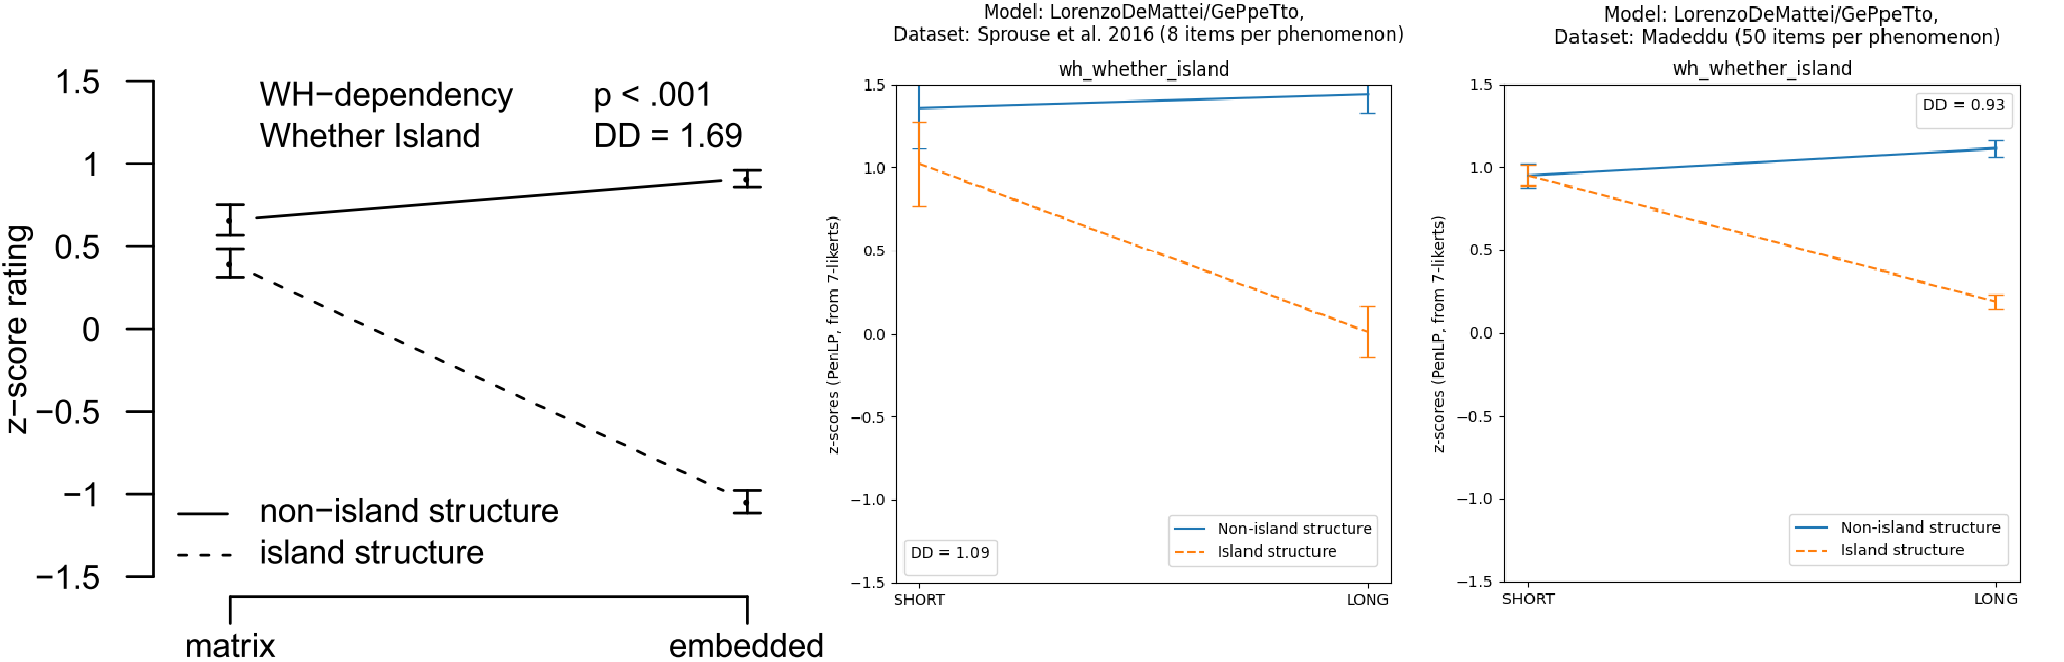
\includegraphics[width=1\textwidth]{images/Chapter1/combined_wh-whether.png} % width= 0.8\textwidth
	\caption{Comparison of wh-dependency whether islands} 
	\label{fig:wh_whether} % this internally labels the figure for future referencing.
	\medskip
	\small
	The first plot on the left shows the scores on humans subjects published in \citet{sprouse2016experimental} for Italian whether islands with wh-dependencies. For each line, the left-most edge represents the score for the short-distance dependency sentence, the right-most the long-distance dependency. The plot in the middle shows the scores from a Gpt-2 model \citep{de2020geppetto} on the same testsuite used for the first plot. The plot on the right shows the scores from the same Gpt-2 models but on the expanded testsuite developed for the present thesis.
\end{figure}

\begin{figure}
	\centering
	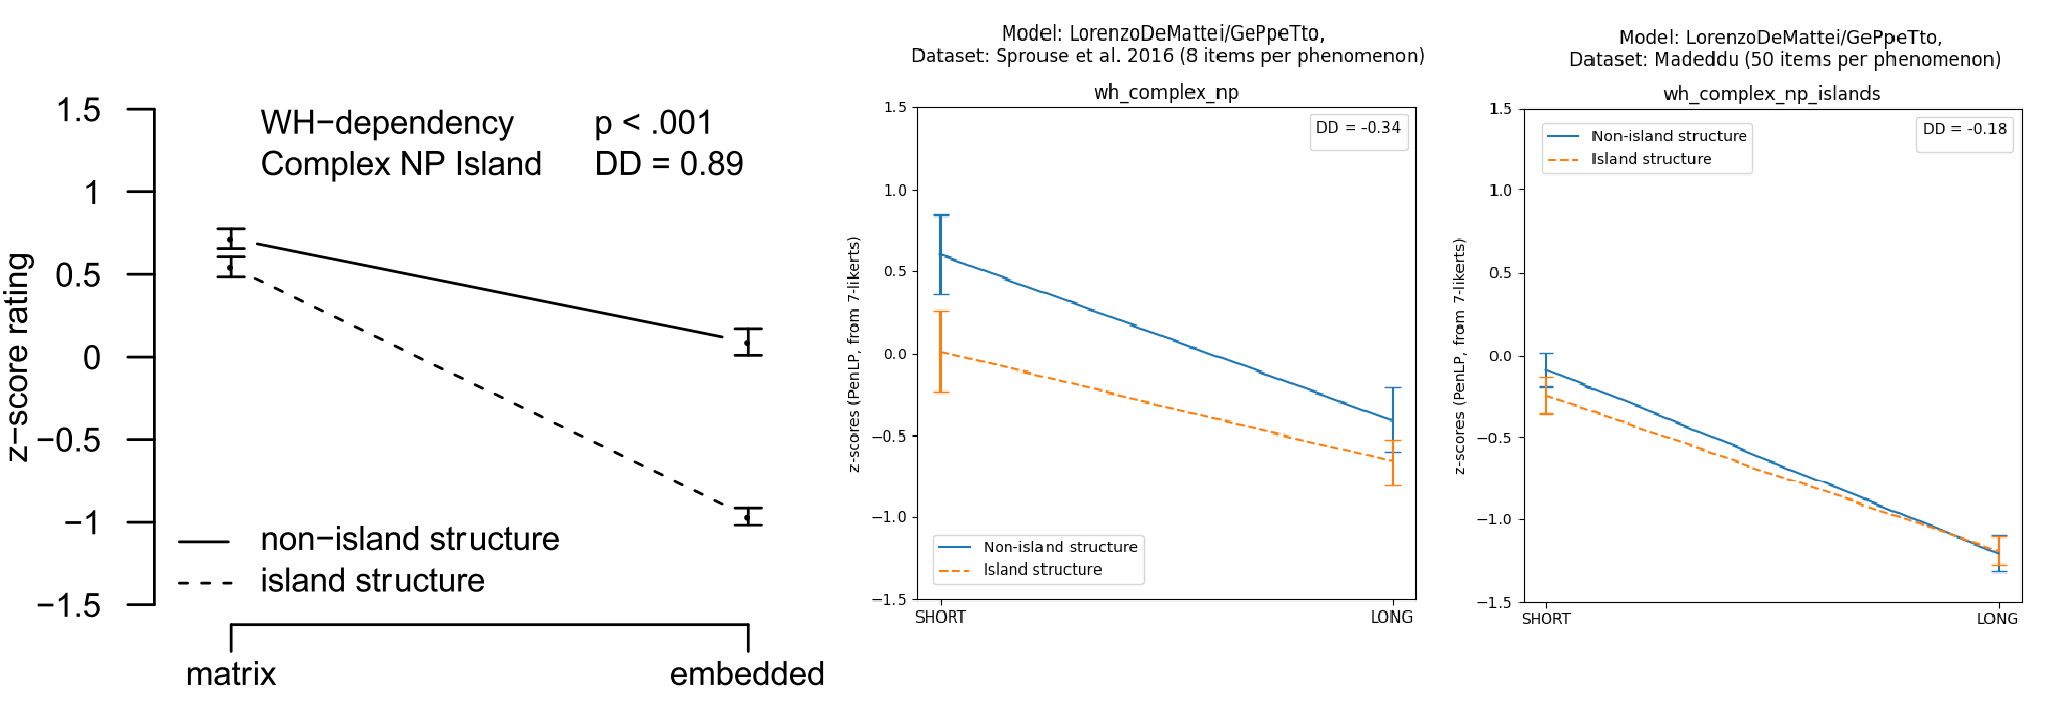
\includegraphics[width=1\textwidth]{images/Chapter1/combined_wh-complex.png} 
	\caption{Comparison of wh-dependencies complex NP islands} 
	\label{fig:wh_complex} % this internally labels the figure for future referencing.
\end{figure}

\begin{figure}
	\centering
	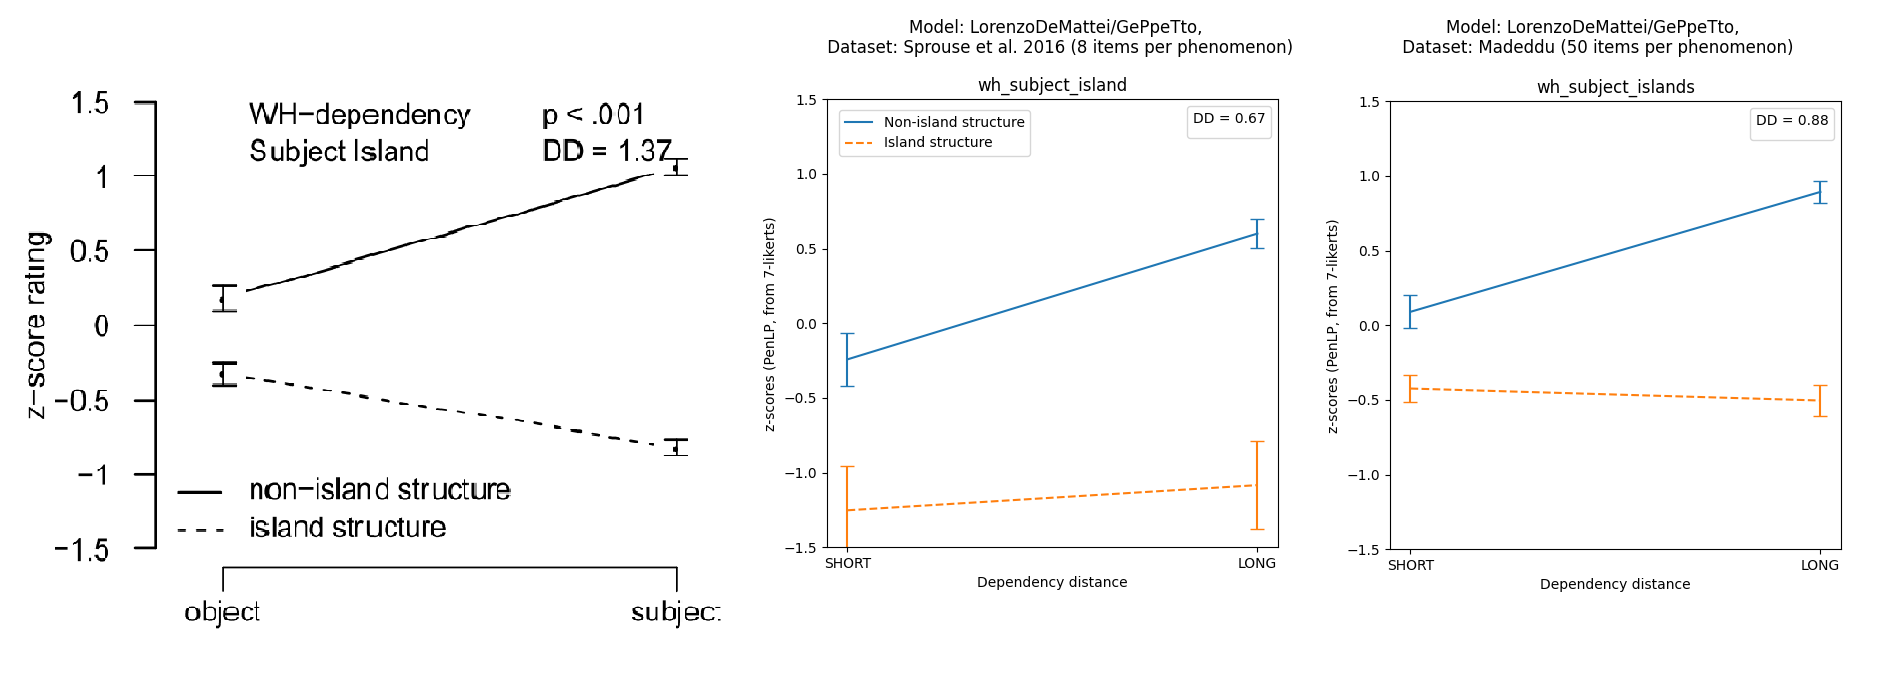
\includegraphics[width=1\textwidth]{images/Chapter1/combined_wh-subject.png} 
	\caption{Comparison of wh-dependencies subject islands} 
	\label{fig:wh_subject} % this internally labels the figure for future referencing.
\end{figure}

\begin{figure}
	\centering
	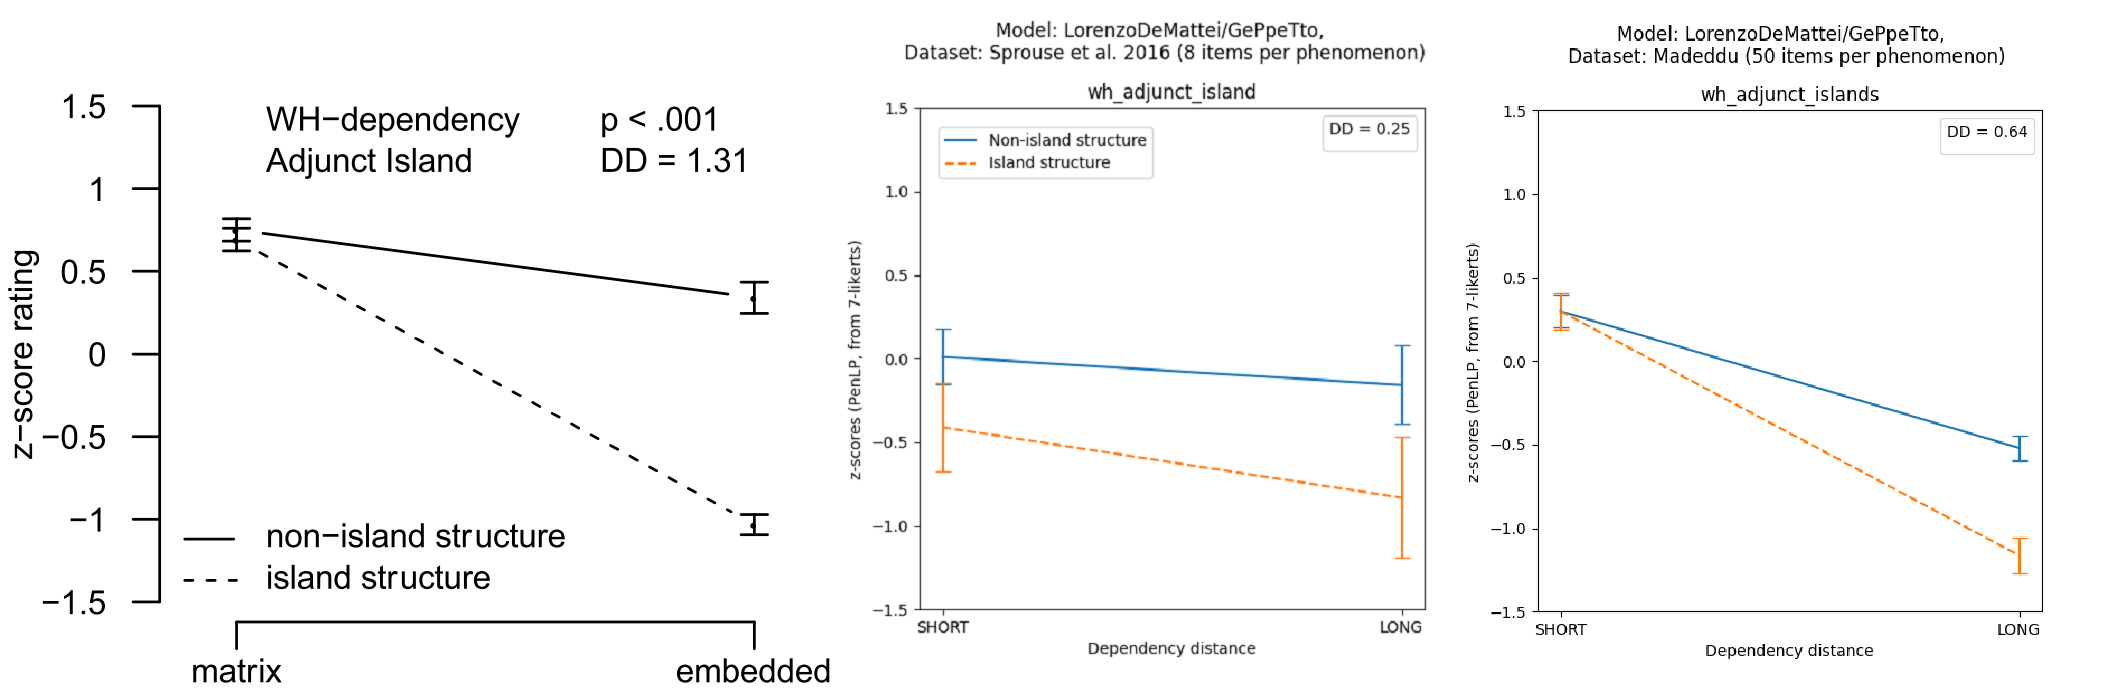
\includegraphics[width=1\textwidth]{images/Chapter1/combined_wh-adjunct.png} 
	\caption{Comparison of wh-dependencies adjunct islands} 
	\label{fig:wh_adjunct} % this internally labels the figure for future referencing.
\end{figure}


Fig.1 Results from Sprouse et al (2016)
Fig.2 Results of acceptability judgements to the same stimuli from Sprouse et al. 2016 from an Italian Gpt-2 model (GePpeTto) with the PenLP acceptability ..score. 
Fig.3

\subsection{Differences between the plots}

..
\subsubsection{Overall}
..
\subsubsection{Whether islands}
..
\subsubsection{Complex np islands}
..
\subsubsection{Subject islands}
..
\subsubsection{Adjunct islands}
..

\subsection{What seems to affect the models acceptability scores}
..
\subsubsection{Whether islands}
..
\subsubsection{Complex np islands}
..
\subsubsection{Subject islands}
..
\subsubsection{Adjunct islands}
..

\subsection{Future work}
..

\subsubsection{This is a sub-subsection}
..



Listing bibliography entries \citep{wei2021frequency, hu2020systematic, lau2020furiously,  sprouse2016experimental}

\subsubsection{This is another subsection}

Quello che segue è un esempio di codice. E' possibile modificare il linguaggio per il synyax highlight, aggiungere parole chiave... E' tutto disponibile nella guida del pacchetto \texttt{listings}.

\lstinputlisting[language=C++]{listings/Capitolo1/code1.cpp} 

\section{Blimp English dataset}
..
\subsection{English models details}
..

\section{Misc notes with refs}

“NATURAL LANGUAGE DOES NOT MAXIMIZE PROBABILITY” 
“Why is human-written text not the most probable text? We conjecture that this is an intrinsic property of human language. Language models that assign probabilities one word at a time without a global model of the text will have trouble capturing this effect. Grice’s Maxims of Communication (Grice, 1975) show that people optimize against stating the obvious. Thus, making every word as predictable as possible will be disfavored. This makes solving the problem simply by training larger models or improving neural architectures using standard per-word learning objectives unlikely: such models are forced to favor the lowest common denominator, rather than informative language.” 
\citep{holtzman2019curious}

Repeated exposure to a type of island construct will increase its perceived acceptability 
\citep{chaves2014subject}

Targed ..syntactic tests on modern language models seem to have started with \citet{linzen2016assessing}, while the use of psycholinguistic tests for this seem to have started with \citet{futrell2018rnns}.


\appendix

\chapter{Factorial design plots}

Scores obtained from the following Huggingface pretrained Italian models:

BERT: dbmdz/bert-base-italian-xxl-cased \footnote{https://huggingface.co/dbmdz/bert-base-italian-xxl-cased} \\
GilBERTo: idb-ita/gilberto-uncased-from-camembert \footnote{https://huggingface.co/idb-ita/gilberto-uncased-from-camembert} \\
GePpeTto: LorenzoDeMattei/GePpeTto \citep{de2020geppetto} \footnote{https://huggingface.co/LorenzoDeMattei/GePpeTto} \\

\clearpage
\section{Sprouse test suite}

\subsection{BERT}

\subsubsection{BERT with PenLP (from softmax model output)}

\begin{figure}[h]
	\centering
	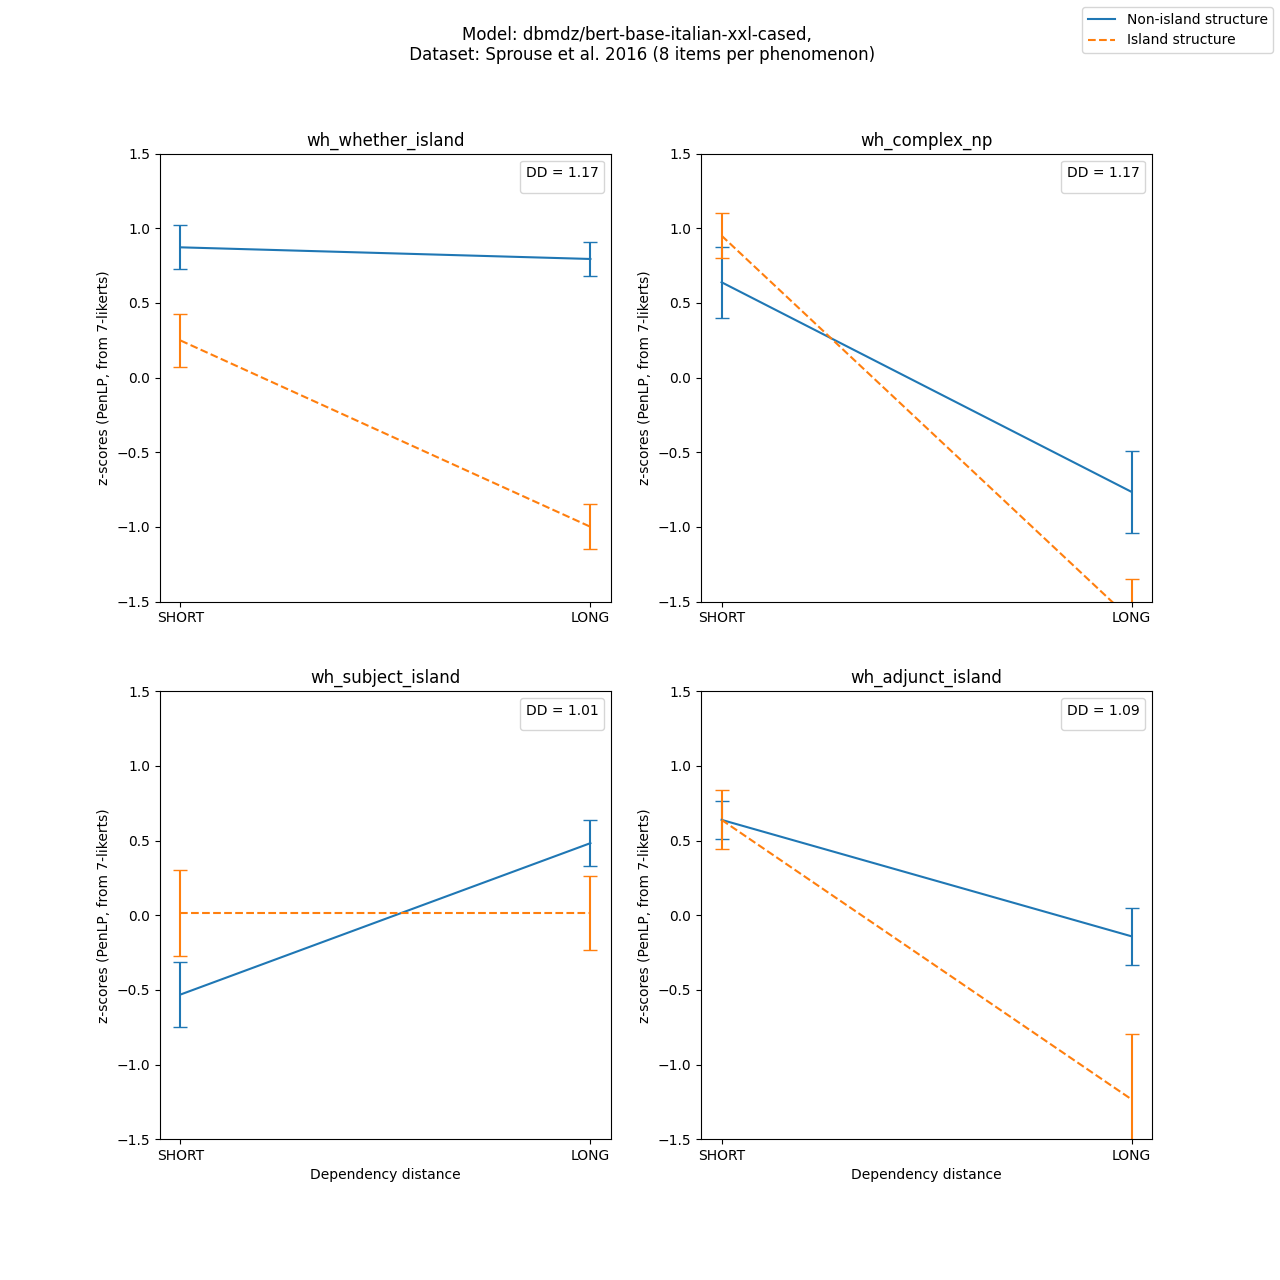
\includegraphics[width=1\textwidth]{images/AppendixA/Sprouse_wh_dbmdz_bert-base-italian-xxl-cased_PenLP-zscores-likert-2022-07-11.png} 
	\label{A-fig:bert_penlp_sprouse}
\end{figure}

\clearpage
\subsubsection{BERT with LP (from softmax model output)}
\begin{figure}[h]
	\centering
	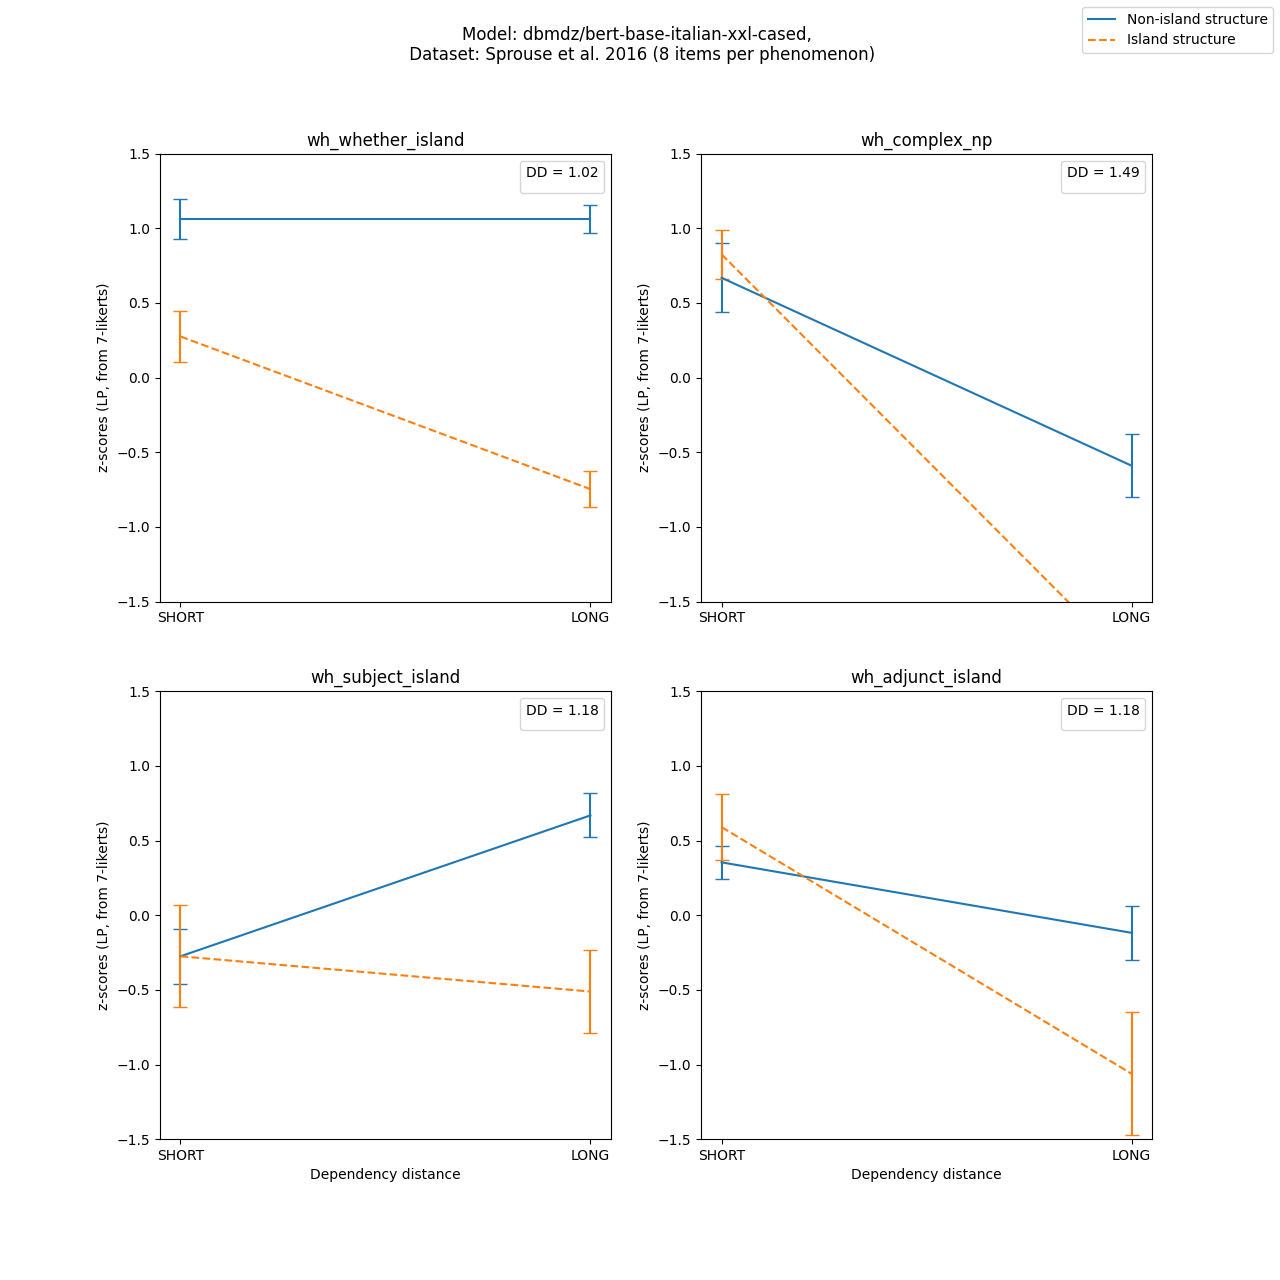
\includegraphics[width=1\textwidth]{images/AppendixA/Sprouse_wh_dbmdz_bert-base-italian-xxl-cased_LP-zscores-likert-2022-07-11.png} 
\end{figure}

\clearpage
\subsubsection{BERT with PenLP-L (from logistic function model output)}

\begin{figure}[h]
	\centering
	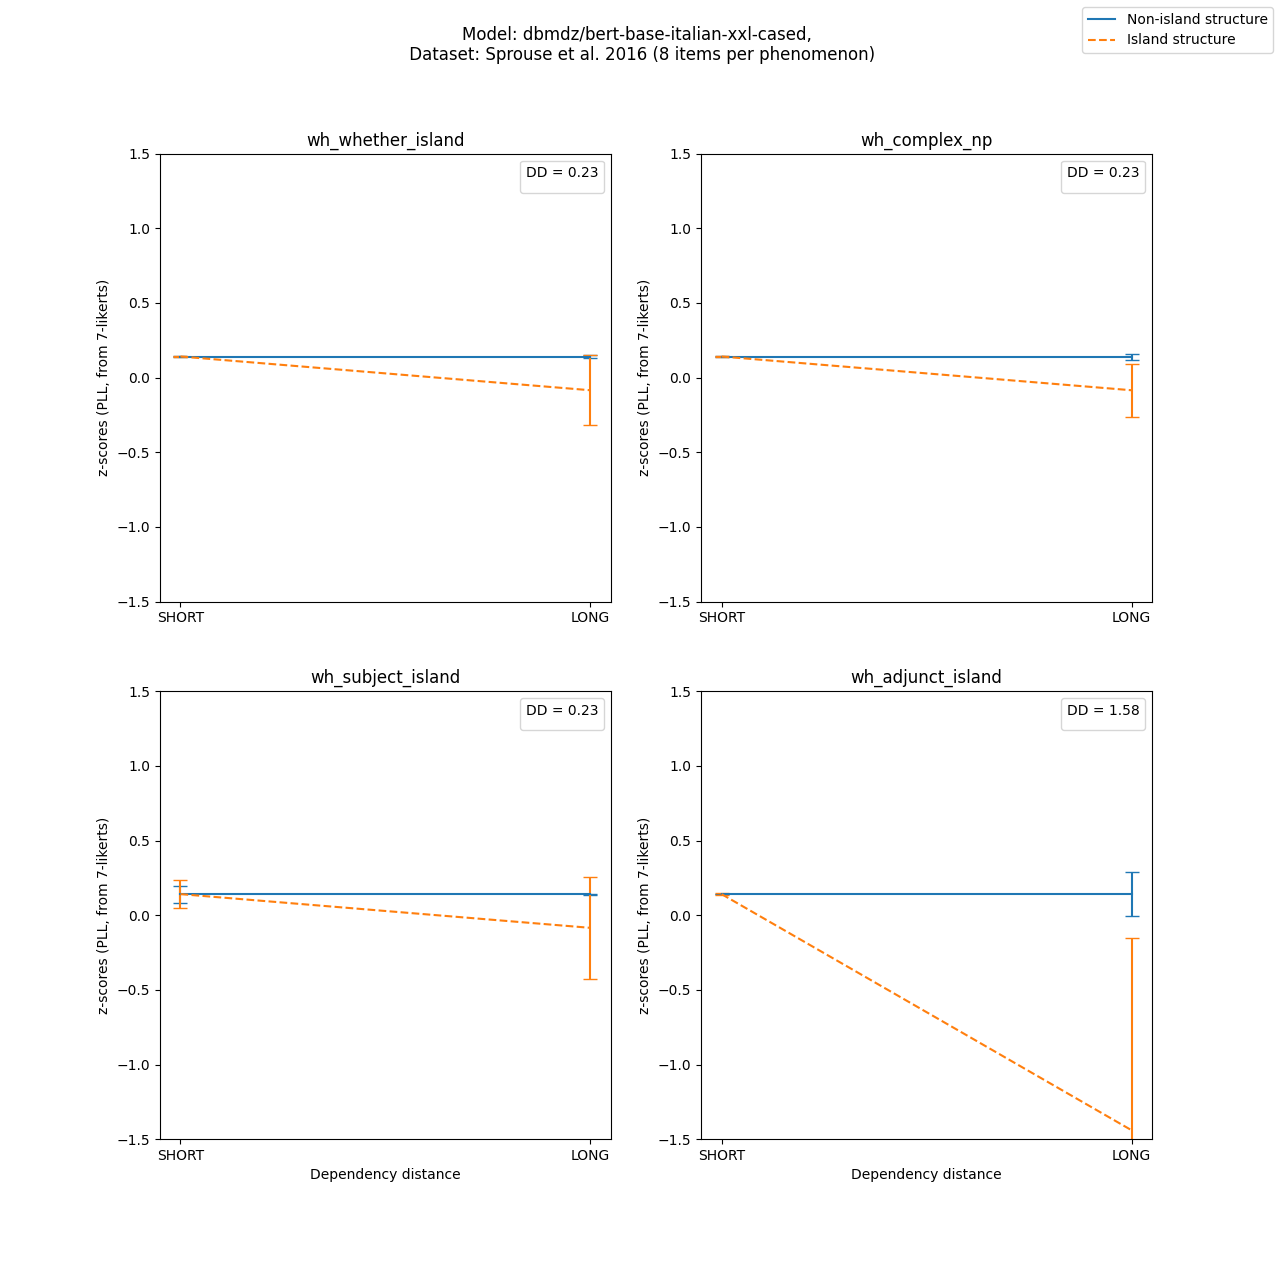
\includegraphics[width=1\textwidth]{images/AppendixA/Sprouse_wh_dbmdz_bert-base-italian-xxl-cased_PLL-zscores-likert-2022-07-11.png} 
\end{figure}

\clearpage
\subsubsection{BERT with LP-L (from logistic function model output)}
\begin{figure}[h]
	\centering
	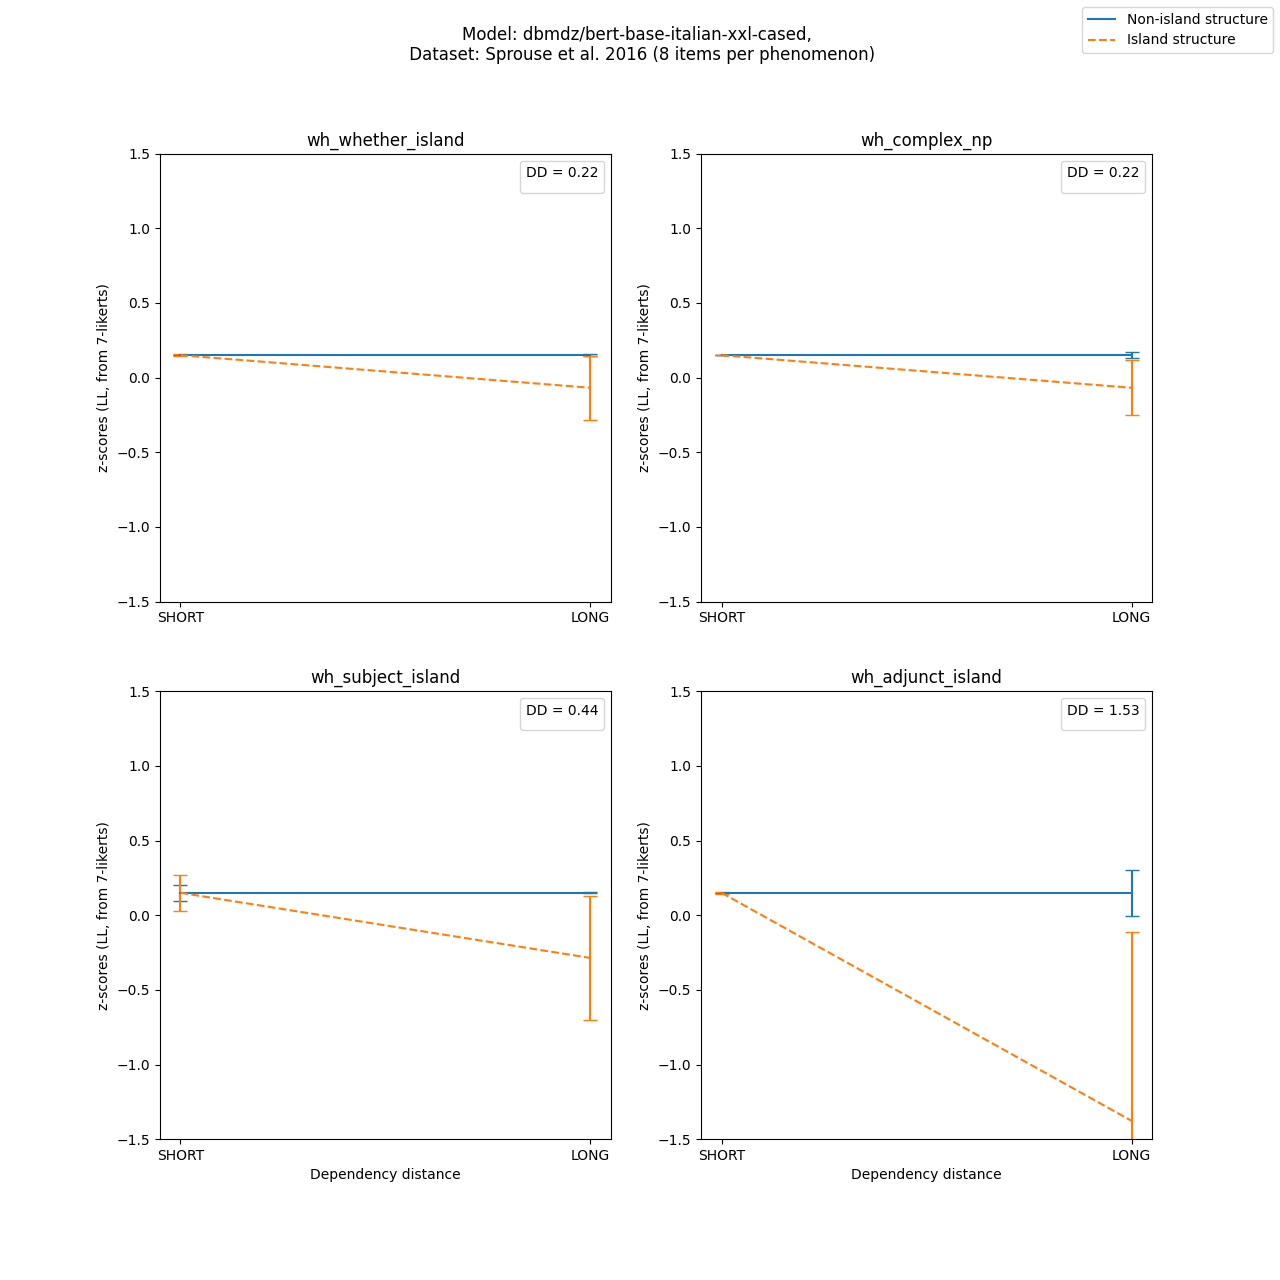
\includegraphics[width=1\textwidth]{images/AppendixA/Sprouse_wh_dbmdz_bert-base-italian-xxl-cased_LL-zscores-likert-2022-07-11.png} 
\end{figure}

\clearpage
\subsection{GilBERTo}

\subsubsection{GilBERTo with PenLP (from softmax model output)}
\begin{figure}[h]
	\centering
	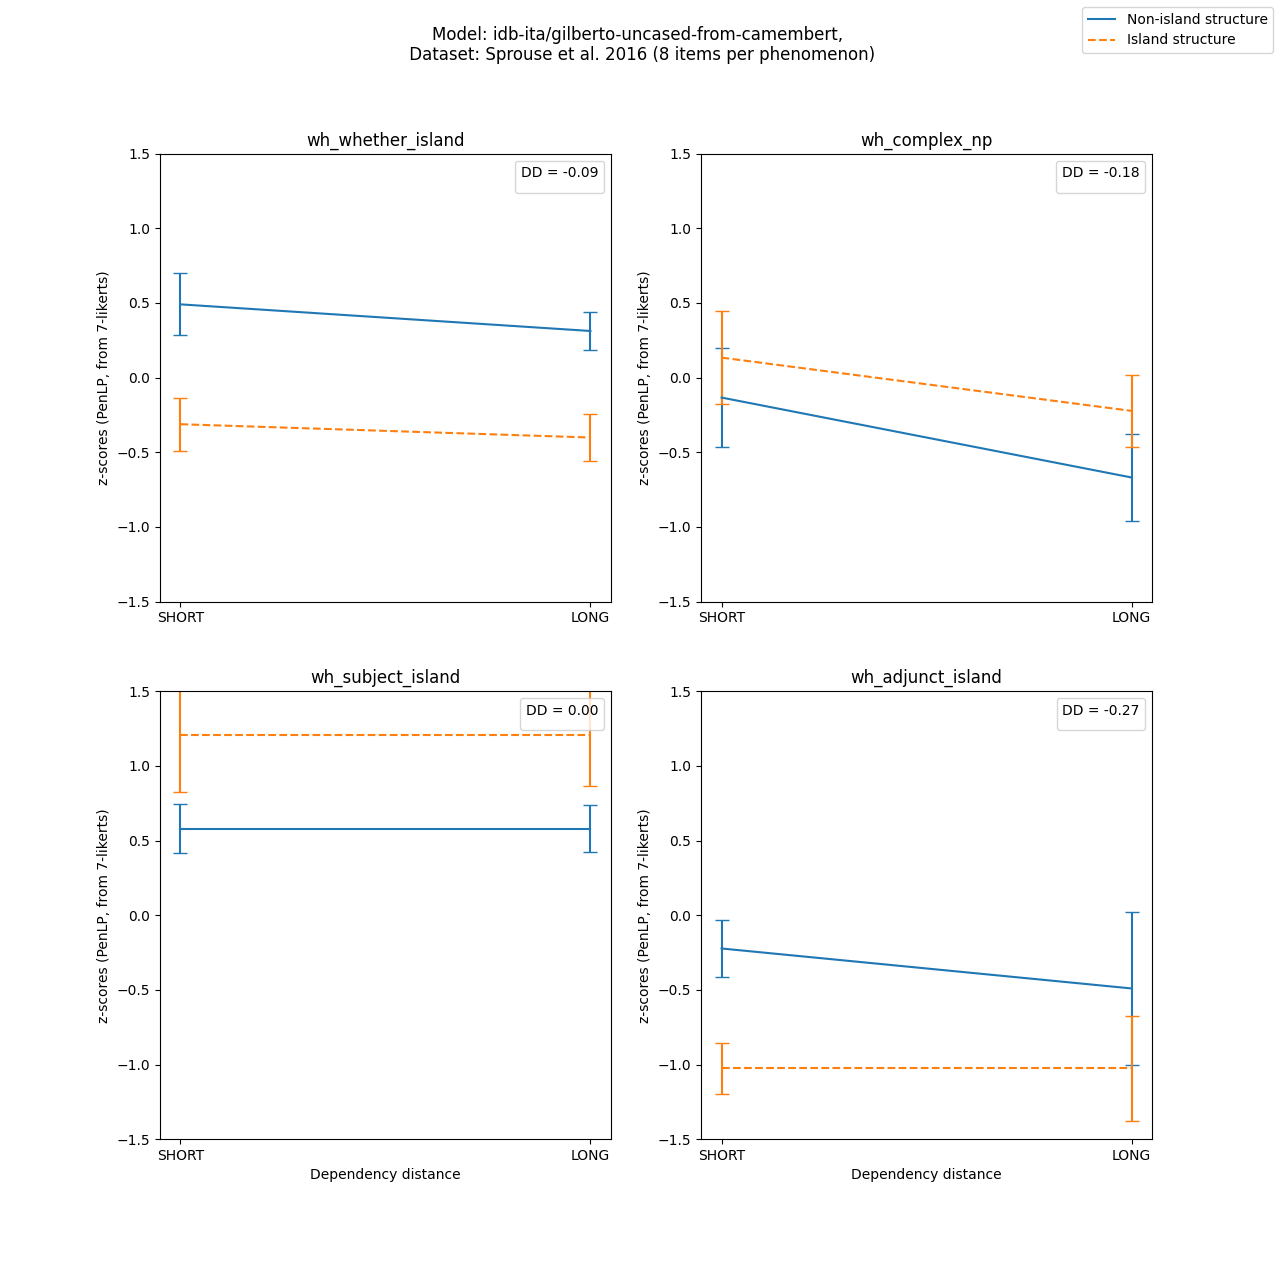
\includegraphics[width=1\textwidth]{images/AppendixA/Sprouse_wh_idb-ita_gilberto-uncased-from-camembert_PenLP-zscores-likert-2022-07-11.png} 
\end{figure}

\clearpage
\subsubsection{GilBERTo with LP (from softmax model output)}
\begin{figure}[h]
	\centering
	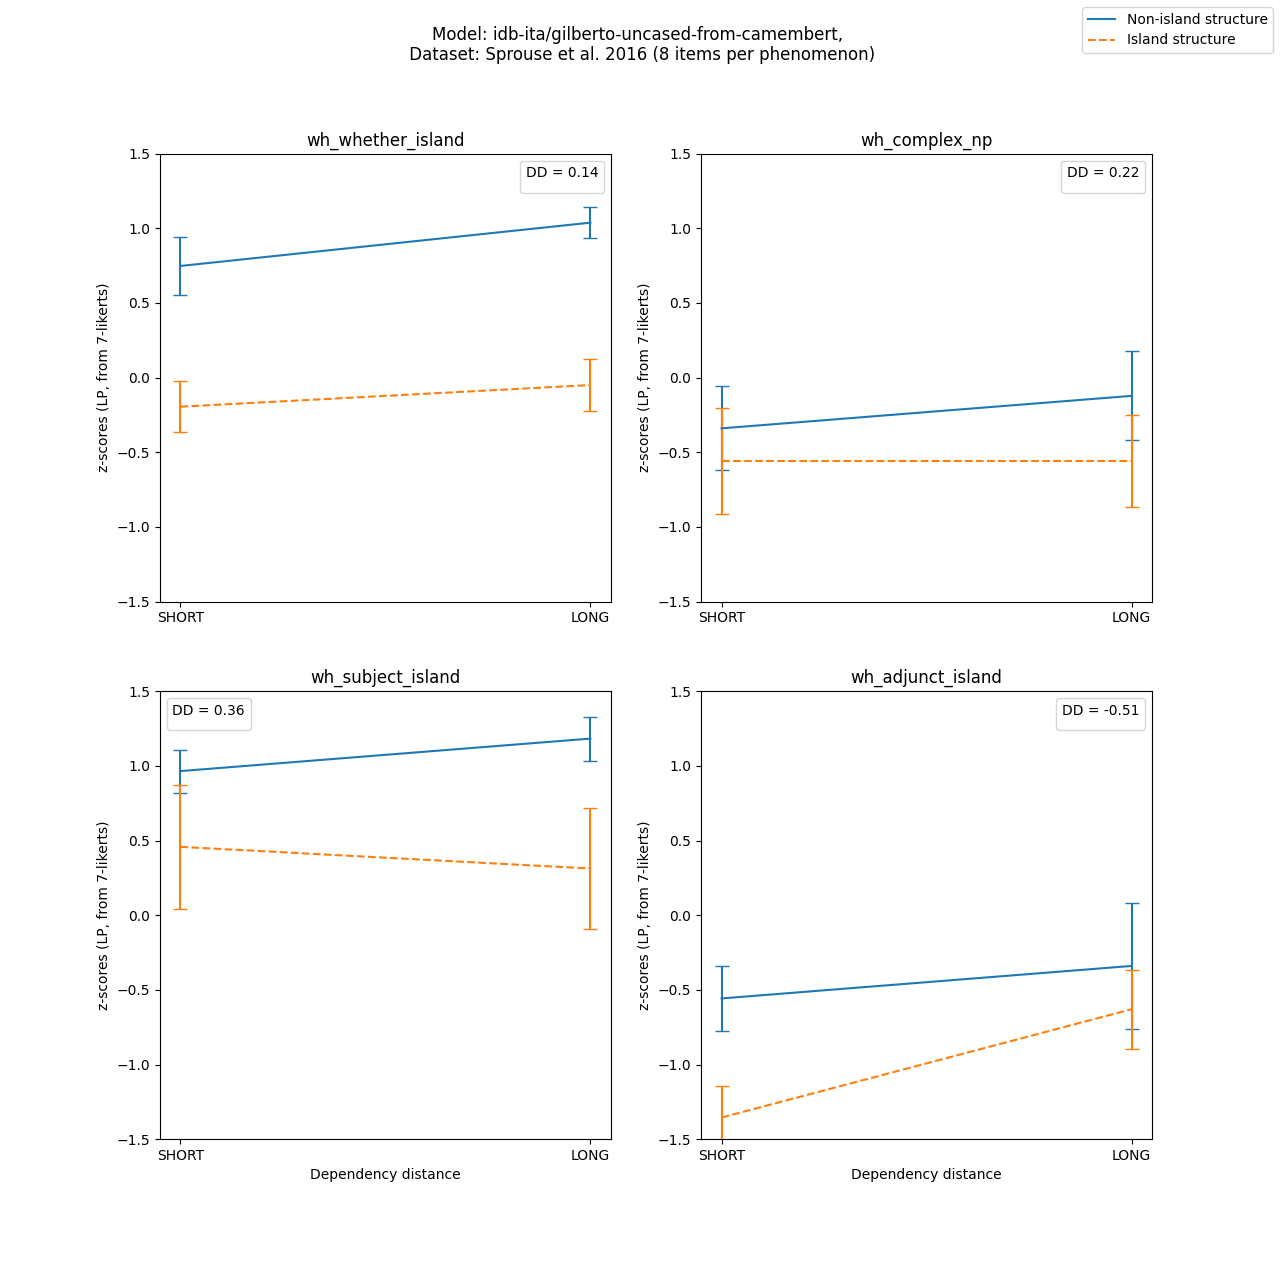
\includegraphics[width=1\textwidth]{images/AppendixA/Sprouse_wh_idb-ita_gilberto-uncased-from-camembert_LP-zscores-likert-2022-07-11.png} 
\end{figure}

\clearpage
\subsubsection{GilBERTo with PenLP-L (from logistic function model output)}
\begin{figure}[h]
	\centering
	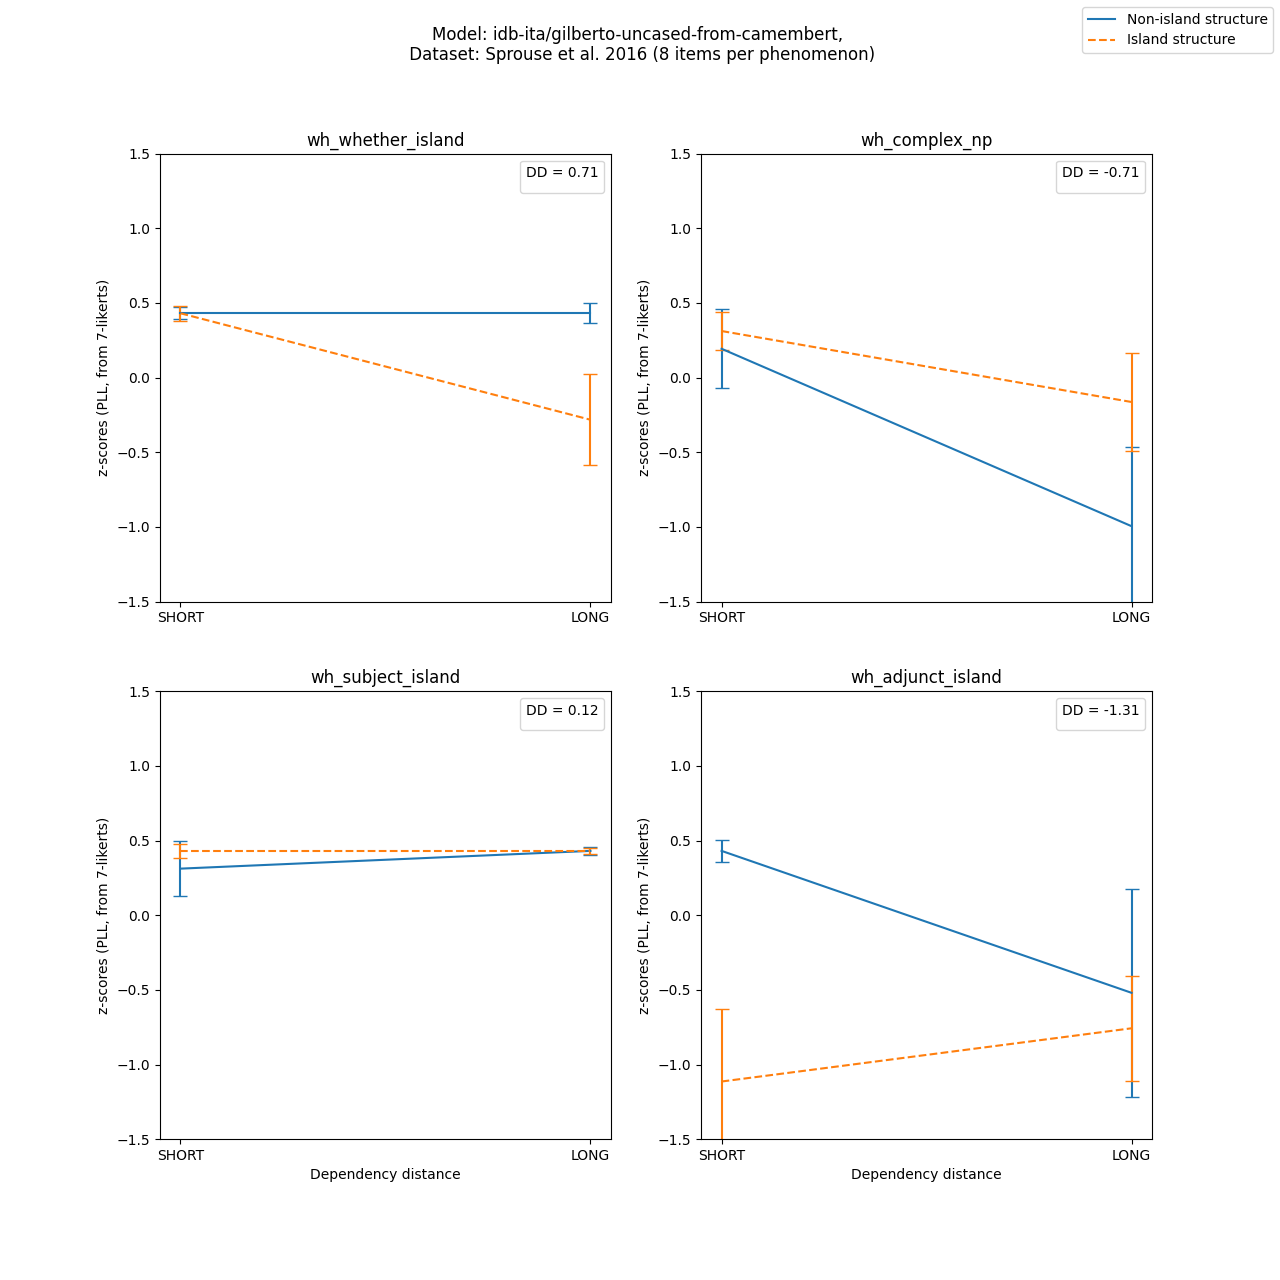
\includegraphics[width=1\textwidth]{images/AppendixA/Sprouse_wh_idb-ita_gilberto-uncased-from-camembert_PLL-zscores-likert-2022-07-11.png} 
\end{figure}

\clearpage
\subsubsection{GilBERTo with LP-L (from logistic function model output)}
\begin{figure}[h]
	\centering
	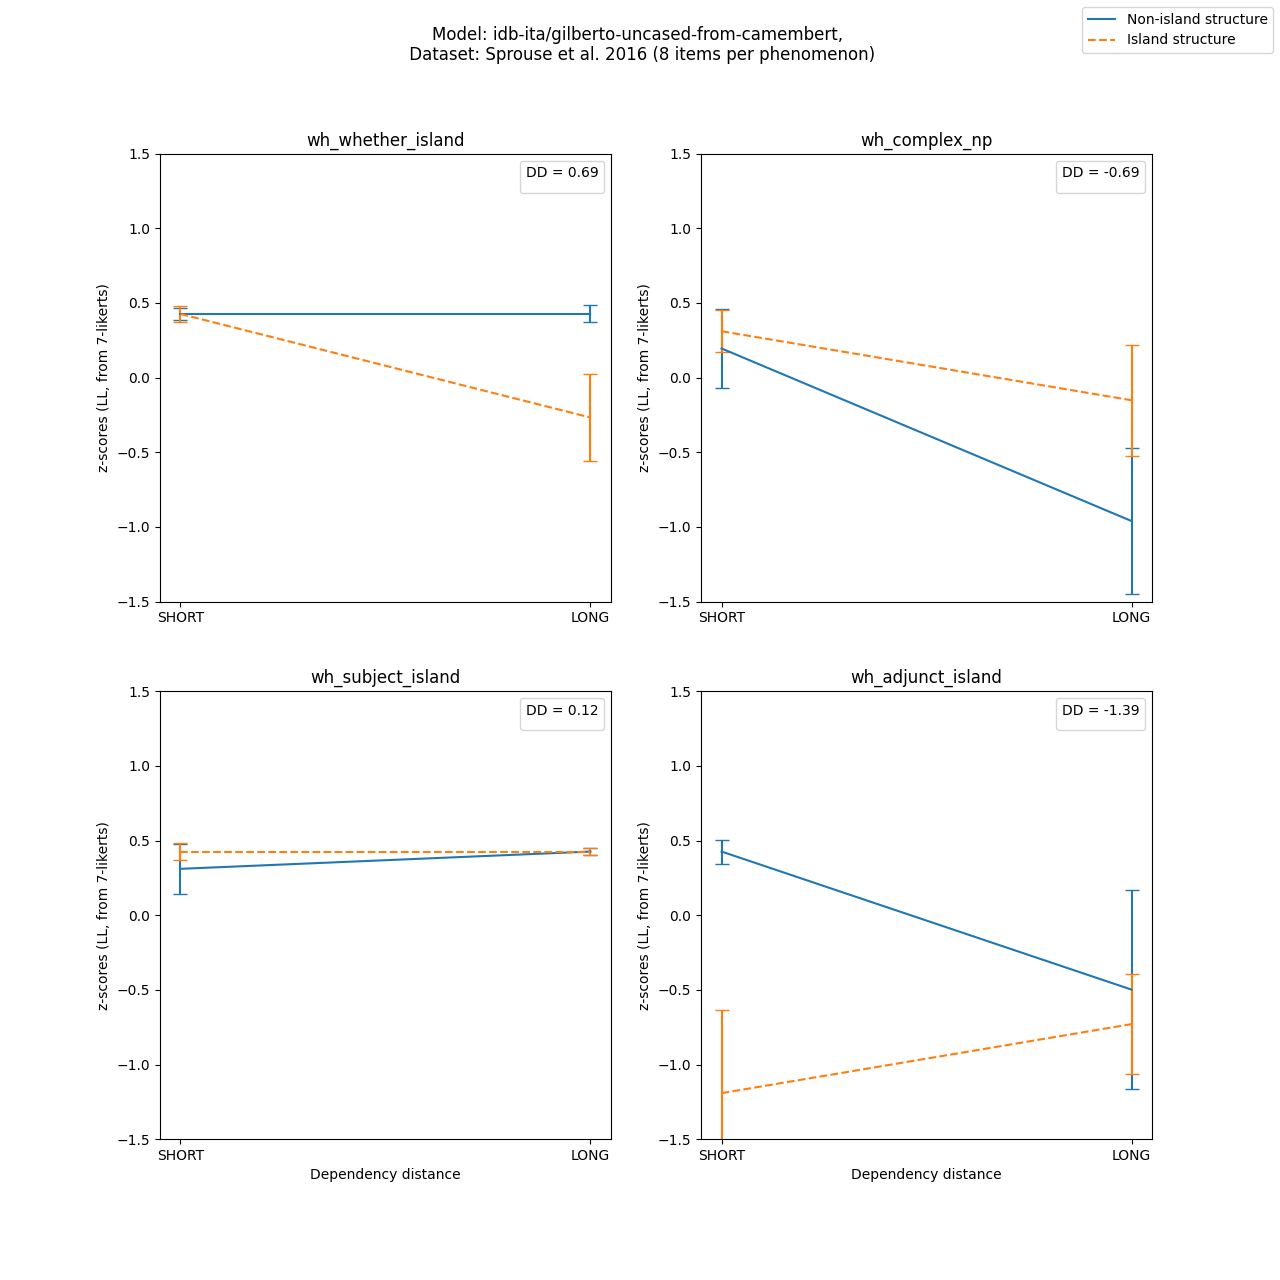
\includegraphics[width=1\textwidth]{images/AppendixA/Sprouse_wh_idb-ita_gilberto-uncased-from-camembert_LL-zscores-likert-2022-07-11.png} 
\end{figure}

\clearpage
\subsection{GePpeTto}

\subsubsection{GePpeTto with PenLP (from softmax model output)}
\begin{figure}[h]
	\centering
	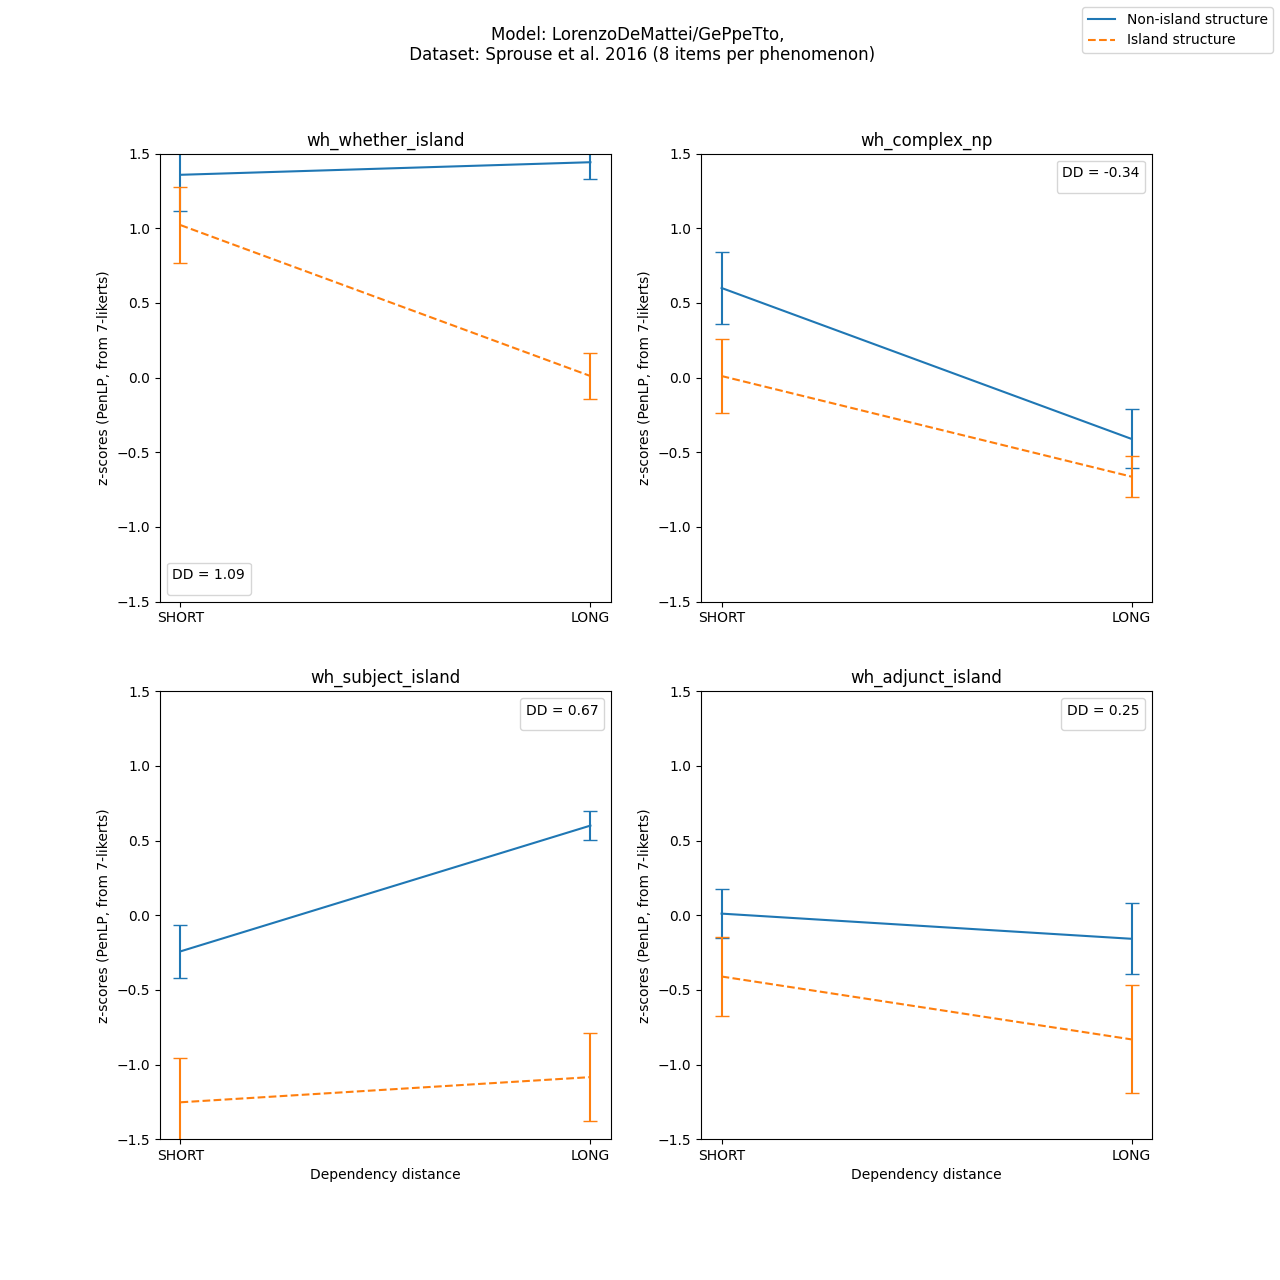
\includegraphics[width=1\textwidth]{images/AppendixA/Sprouse_wh_LorenzoDeMattei_GePpeTto_PenLP-zscores-likert-2022-07-11.png} 
\end{figure}

\clearpage
\subsubsection{GePpeTto with LP (from softmax model output)}
\begin{figure}[h]
	\centering
	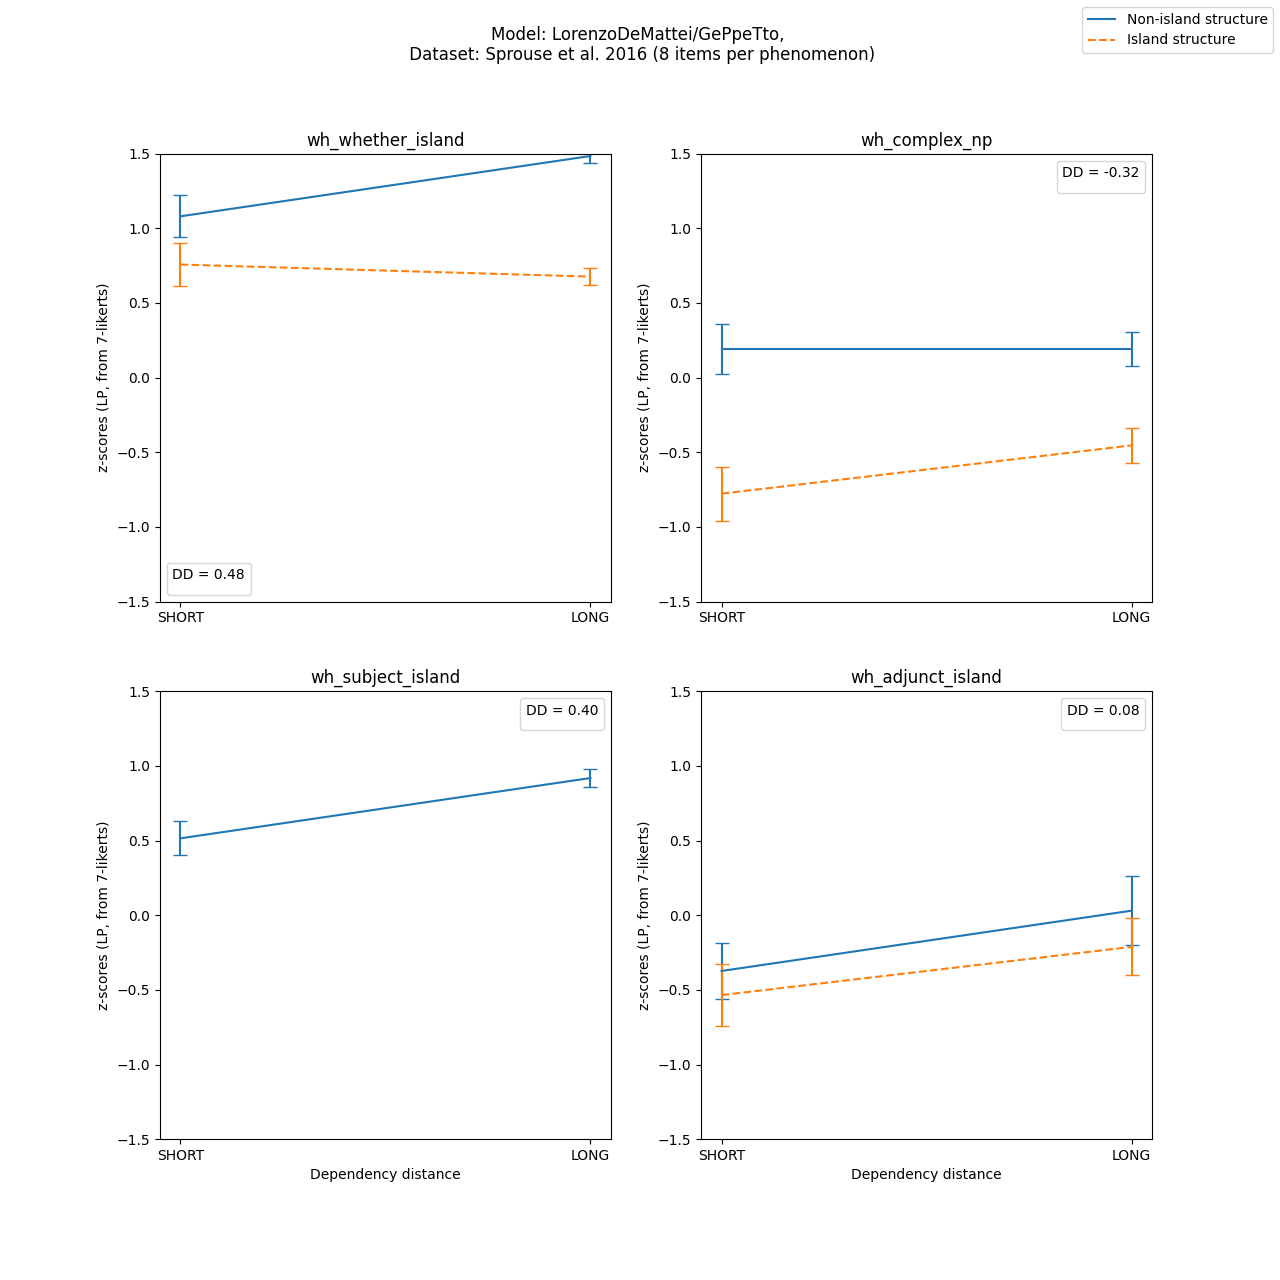
\includegraphics[width=1\textwidth]{images/AppendixA/Sprouse_wh_LorenzoDeMattei_GePpeTto_LP-zscores-likert-2022-07-11.png} 
\end{figure}

\clearpage
\section{Madeddu test suite}

\subsection{BERT}

\subsubsection{BERT with PenLP (from softmax model output)}
\begin{figure}[h]
	\centering
	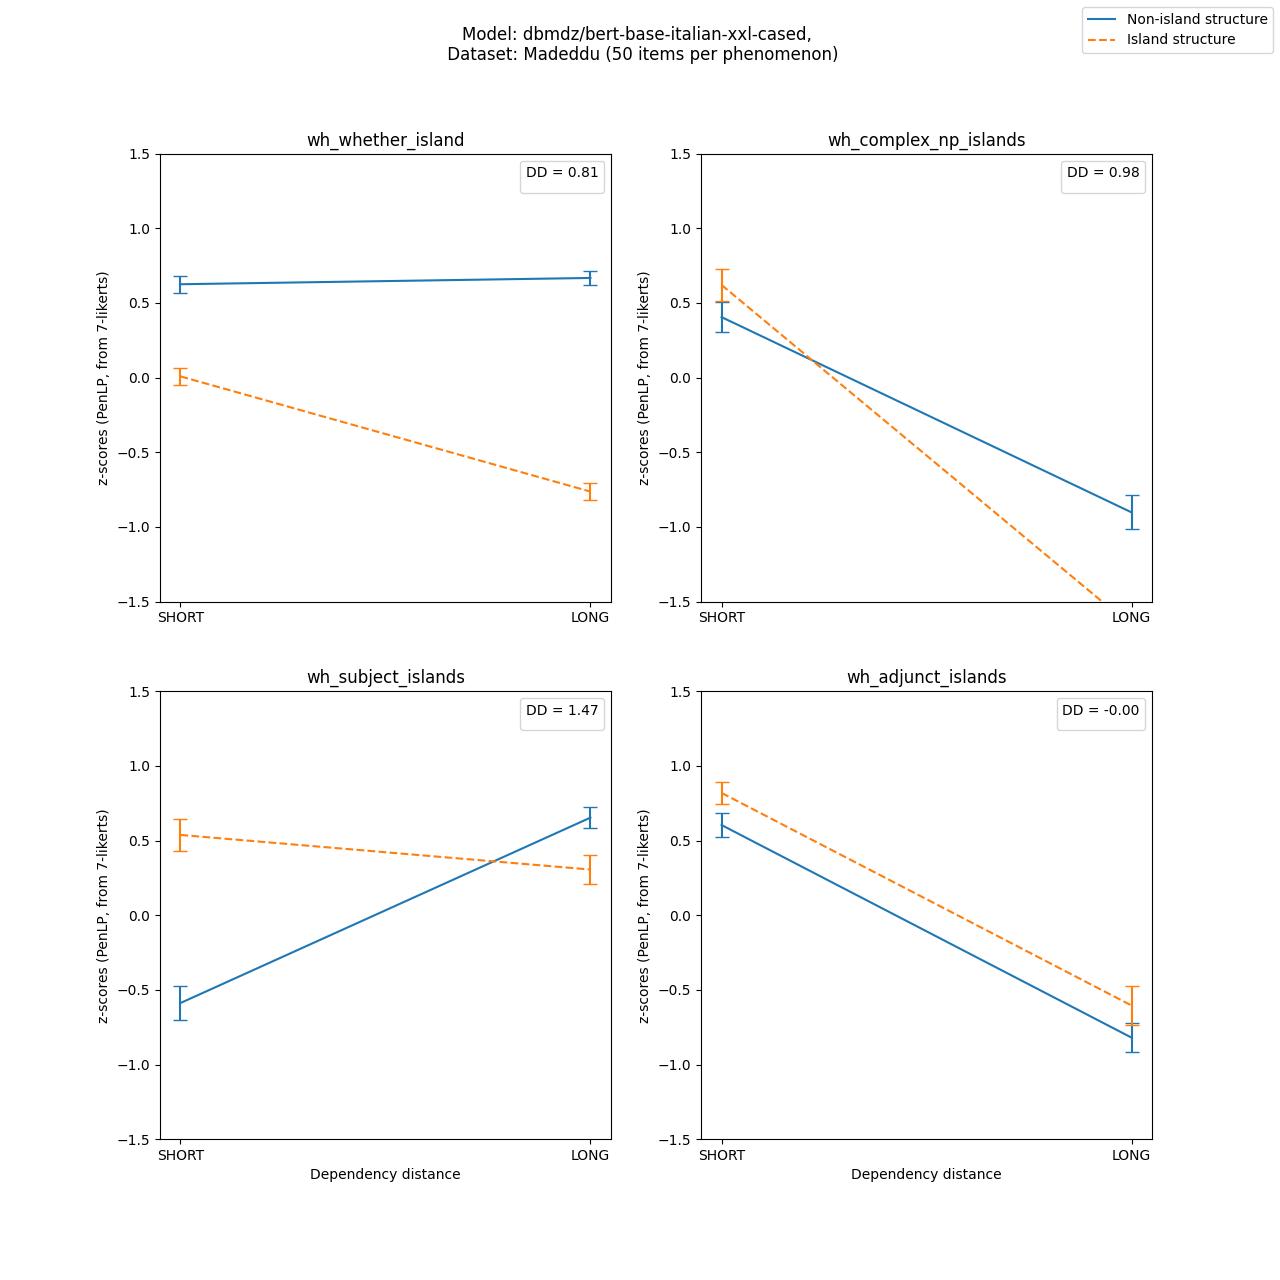
\includegraphics[width=1\textwidth]{images/AppendixA/Madeddu_wh_dbmdz_bert-base-italian-xxl-cased_PenLP-zscores-likert-2022-07-11.png} 
\end{figure}

\clearpage
\subsubsection{BERT with LP (from softmax model output)}
\begin{figure}[h]
	\centering
	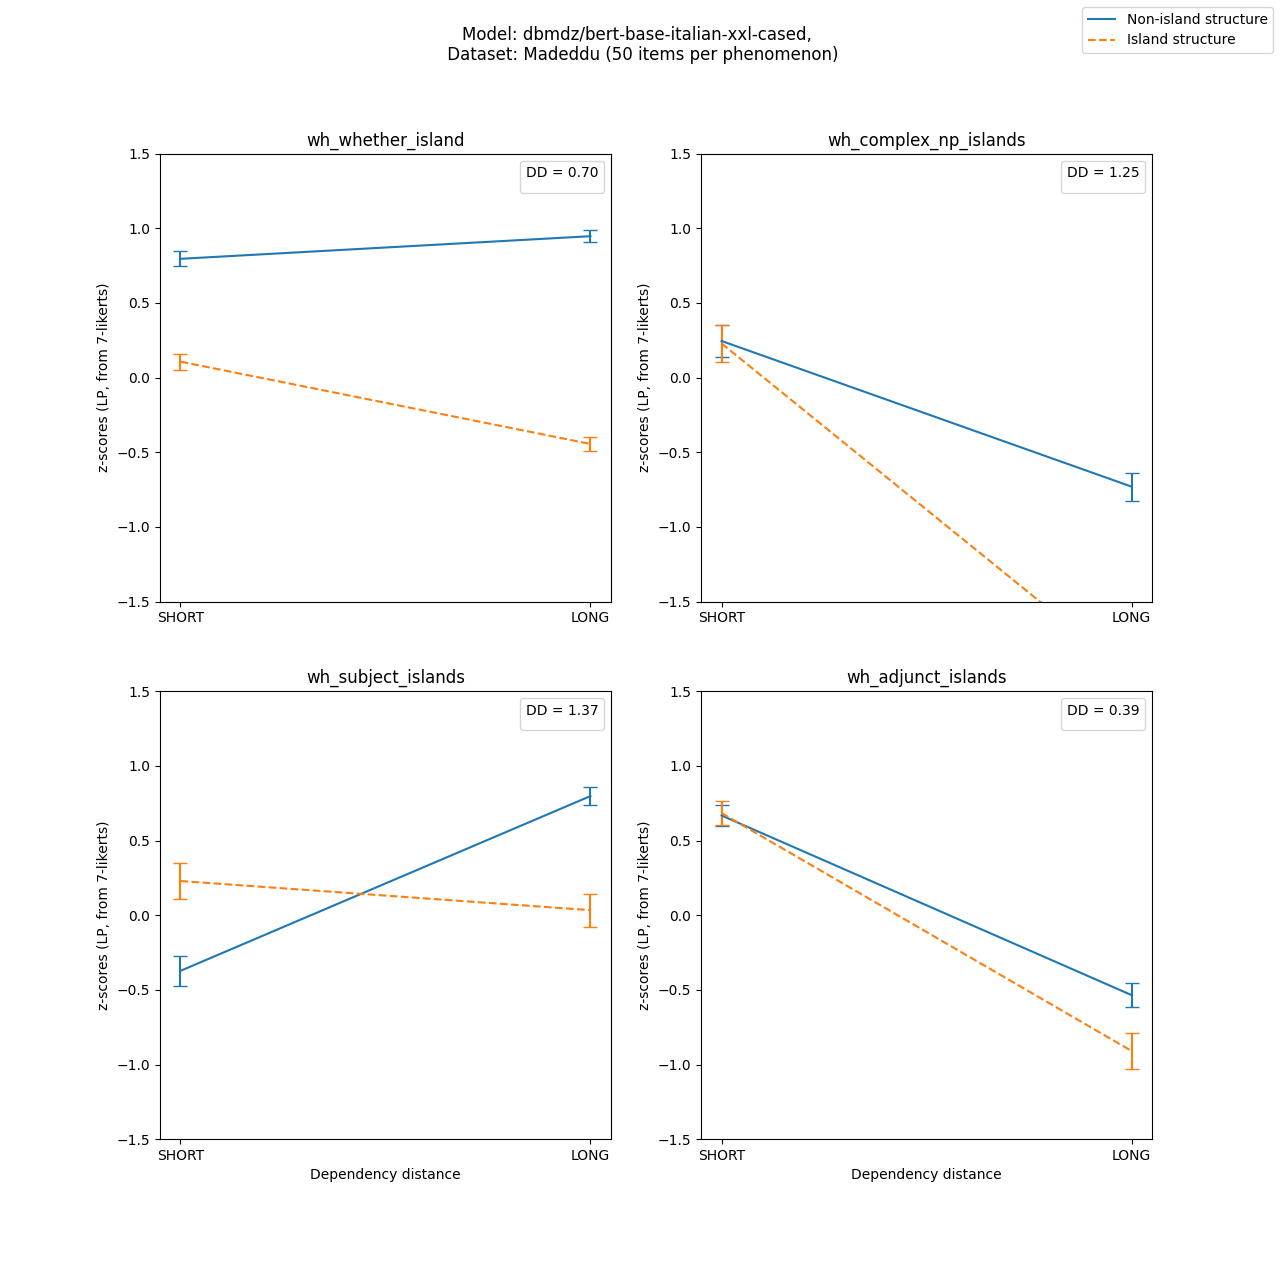
\includegraphics[width=1\textwidth]{images/AppendixA/Madeddu_wh_dbmdz_bert-base-italian-xxl-cased_LP-zscores-likert-2022-07-11.png} 
\end{figure}

\clearpage
\subsubsection{BERT with PenLP-L (from logistic function model output)}
\begin{figure}[h]
	\centering
	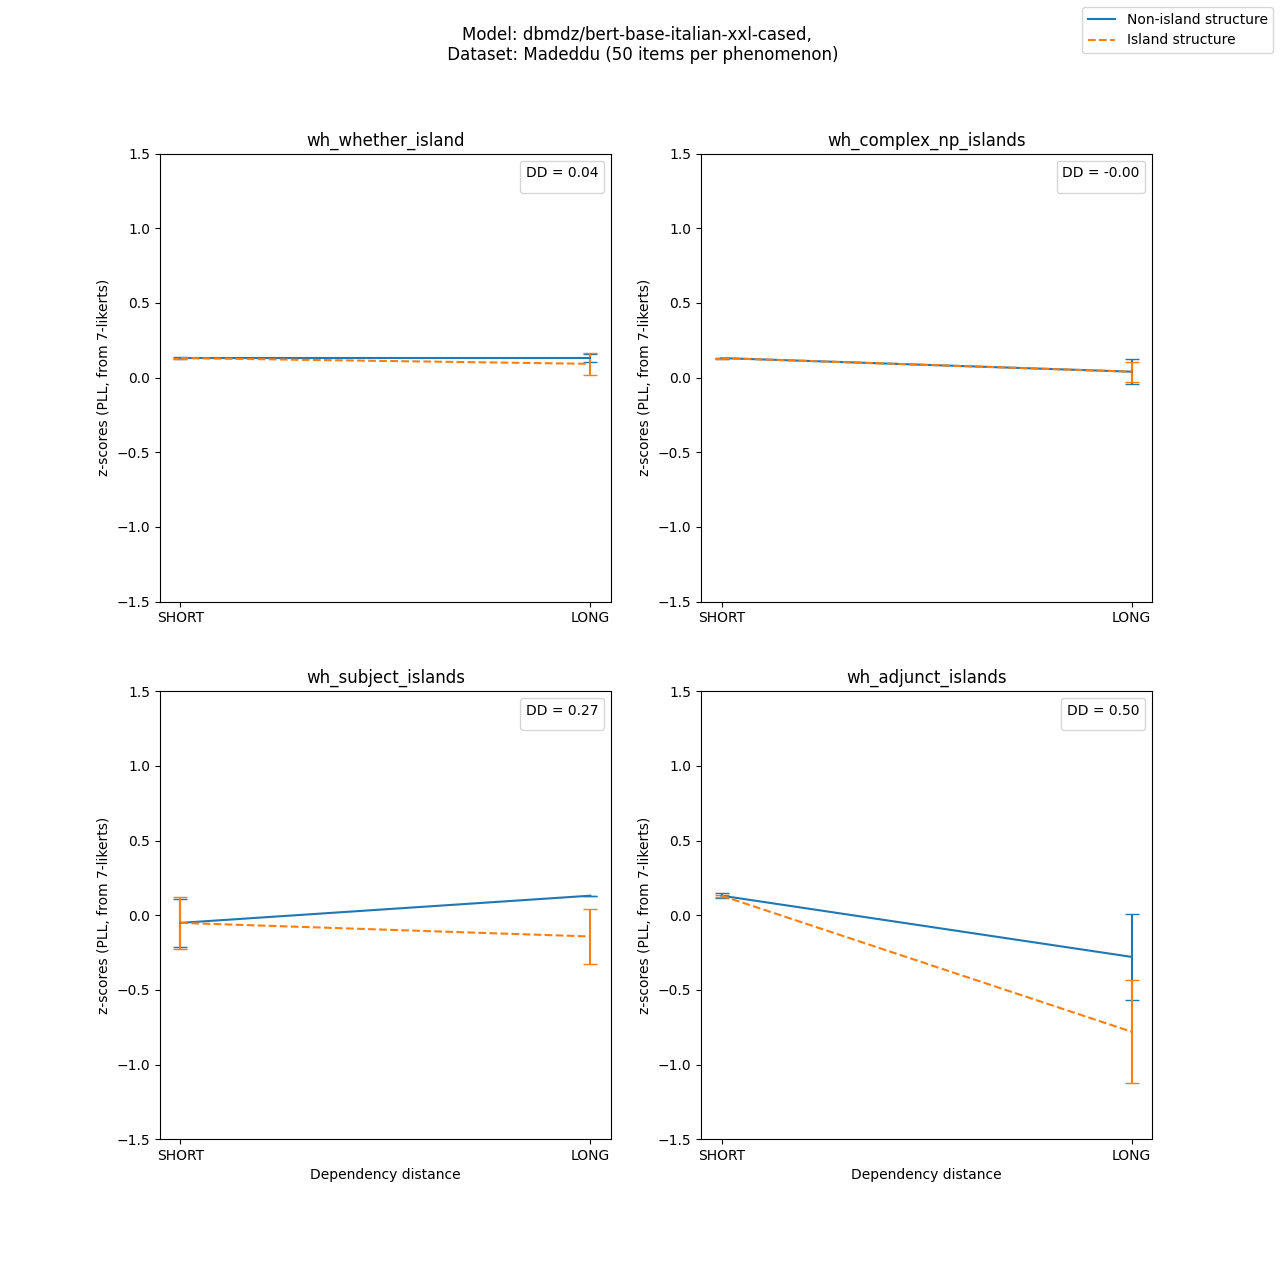
\includegraphics[width=1\textwidth]{images/AppendixA/Madeddu_wh_dbmdz_bert-base-italian-xxl-cased_PLL-zscores-likert-2022-07-11.png} 
\end{figure}

\clearpage
\subsubsection{BERT with LP-L (from logistic function model output)}
\begin{figure}[h]
	\centering
	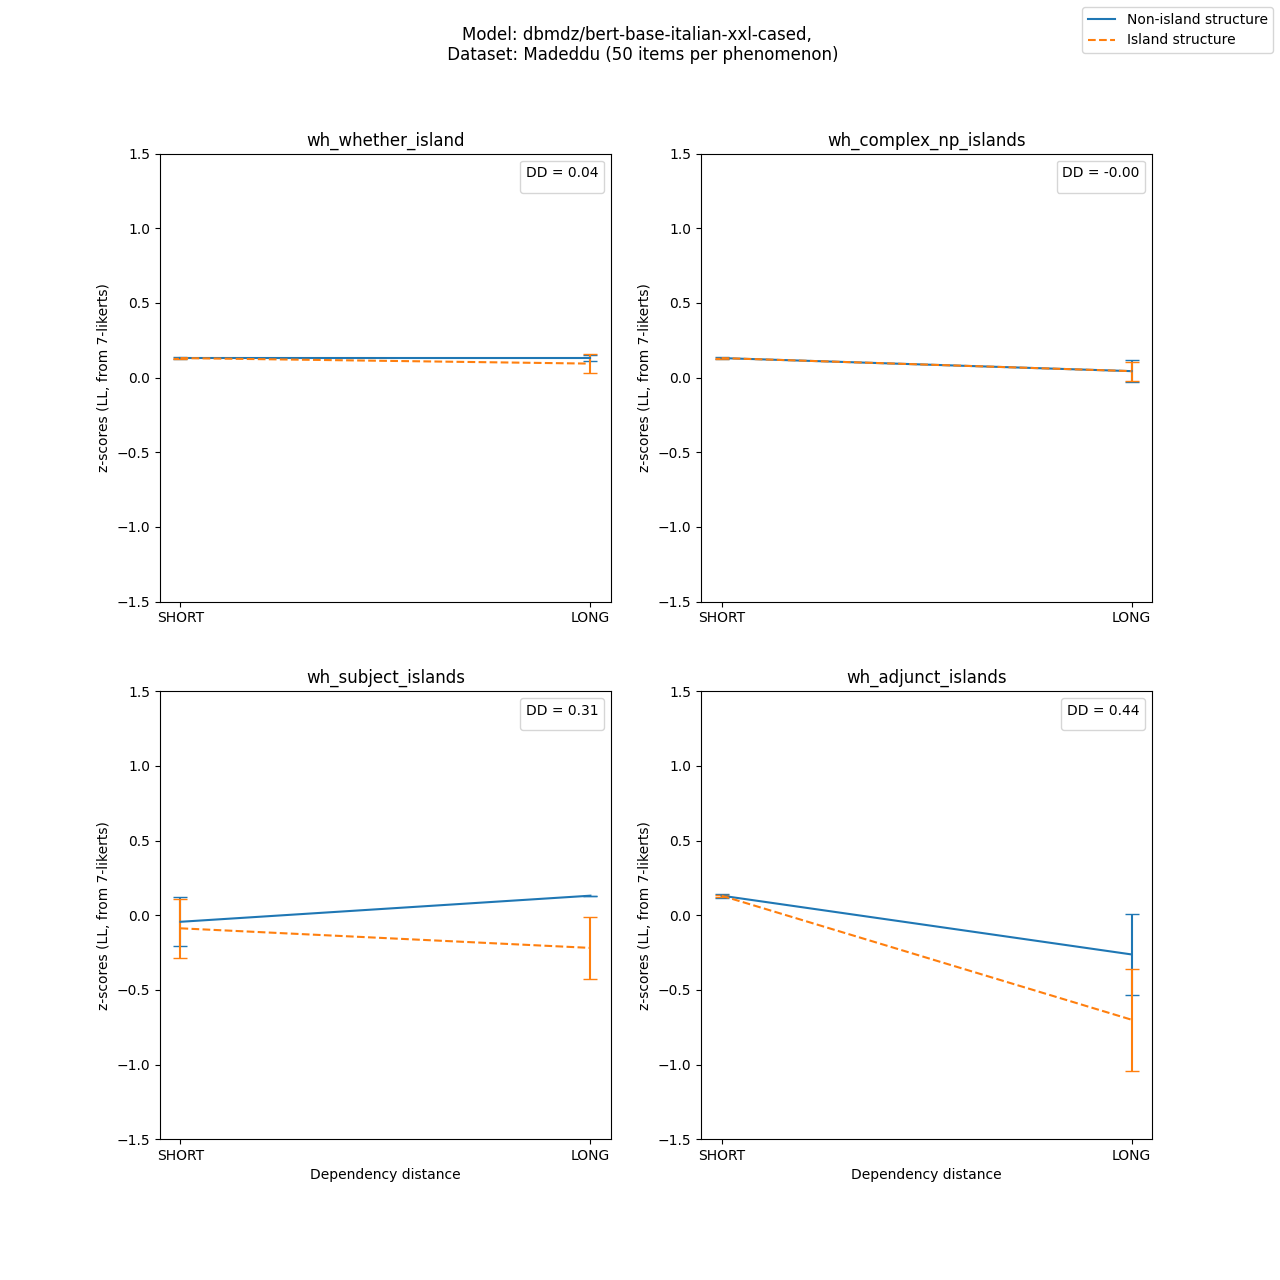
\includegraphics[width=1\textwidth]{images/AppendixA/Madeddu_wh_dbmdz_bert-base-italian-xxl-cased_LL-zscores-likert-2022-07-11.png} 
\end{figure}

\clearpage
\subsection{GilBERTo}

\subsubsection{GilBERTo with PenLP (from softmax model output)}
\begin{figure}[h]
	\centering
	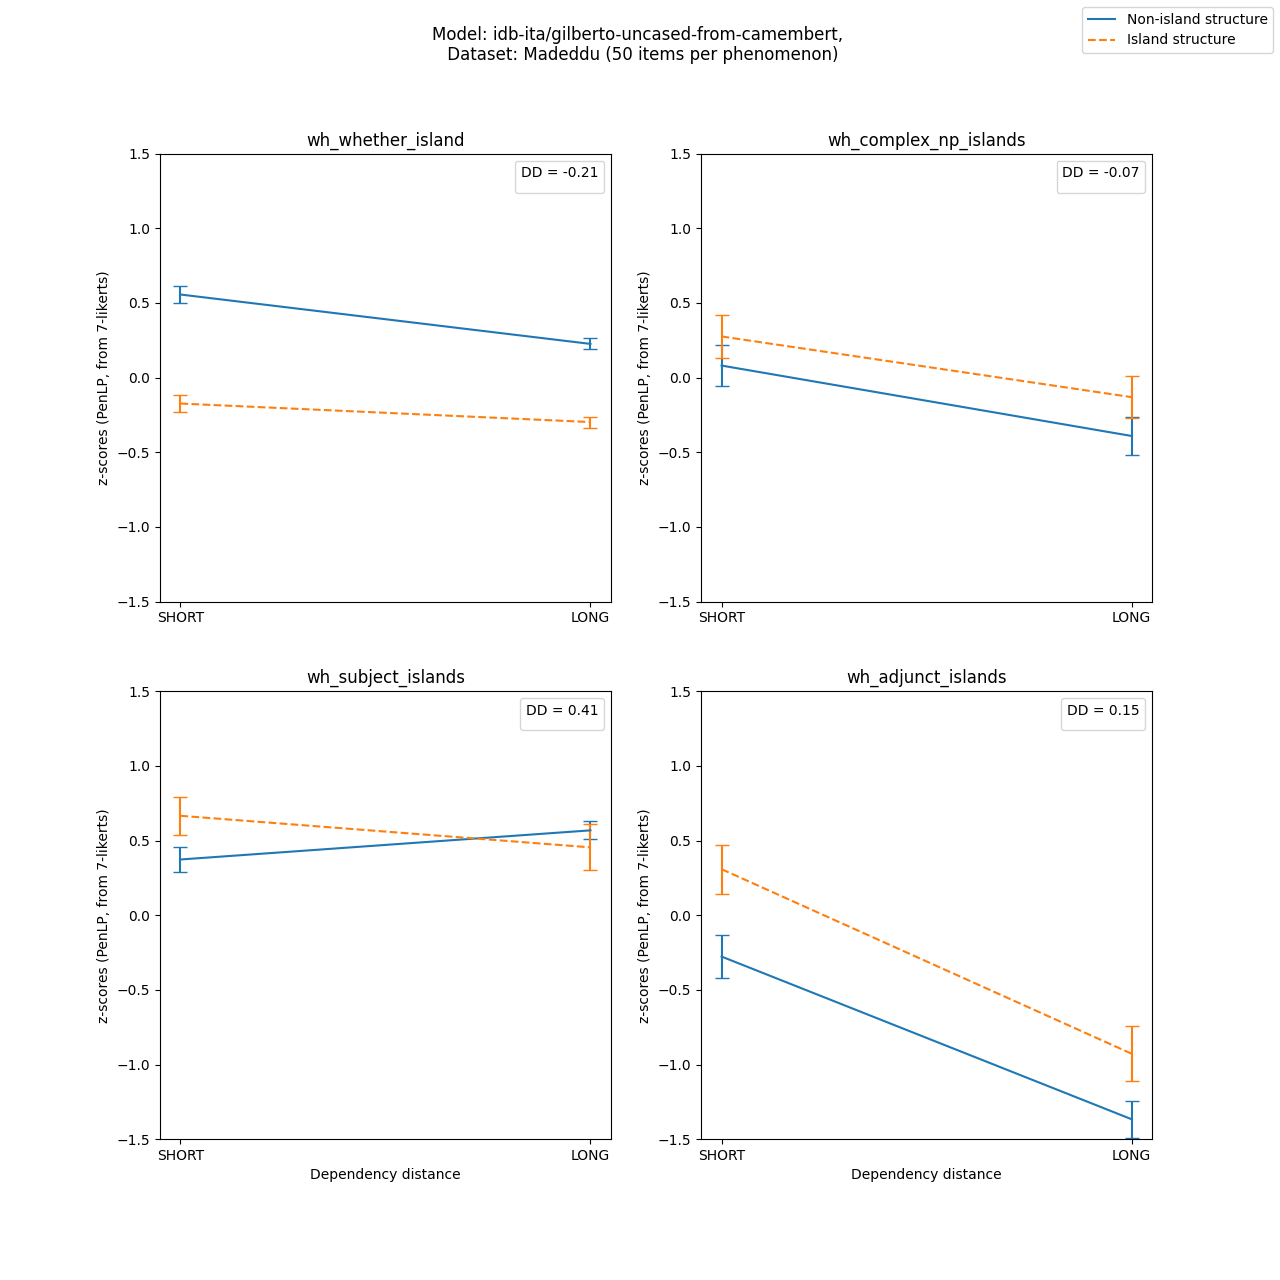
\includegraphics[width=1\textwidth]{images/AppendixA/Madeddu_wh_idb-ita_gilberto-uncased-from-camembert_PenLP-zscores-likert-2022-07-11.png} 
\end{figure}

\clearpage
\subsubsection{GilBERTo with LP (from softmax model output)}
\begin{figure}[h]
	\centering
	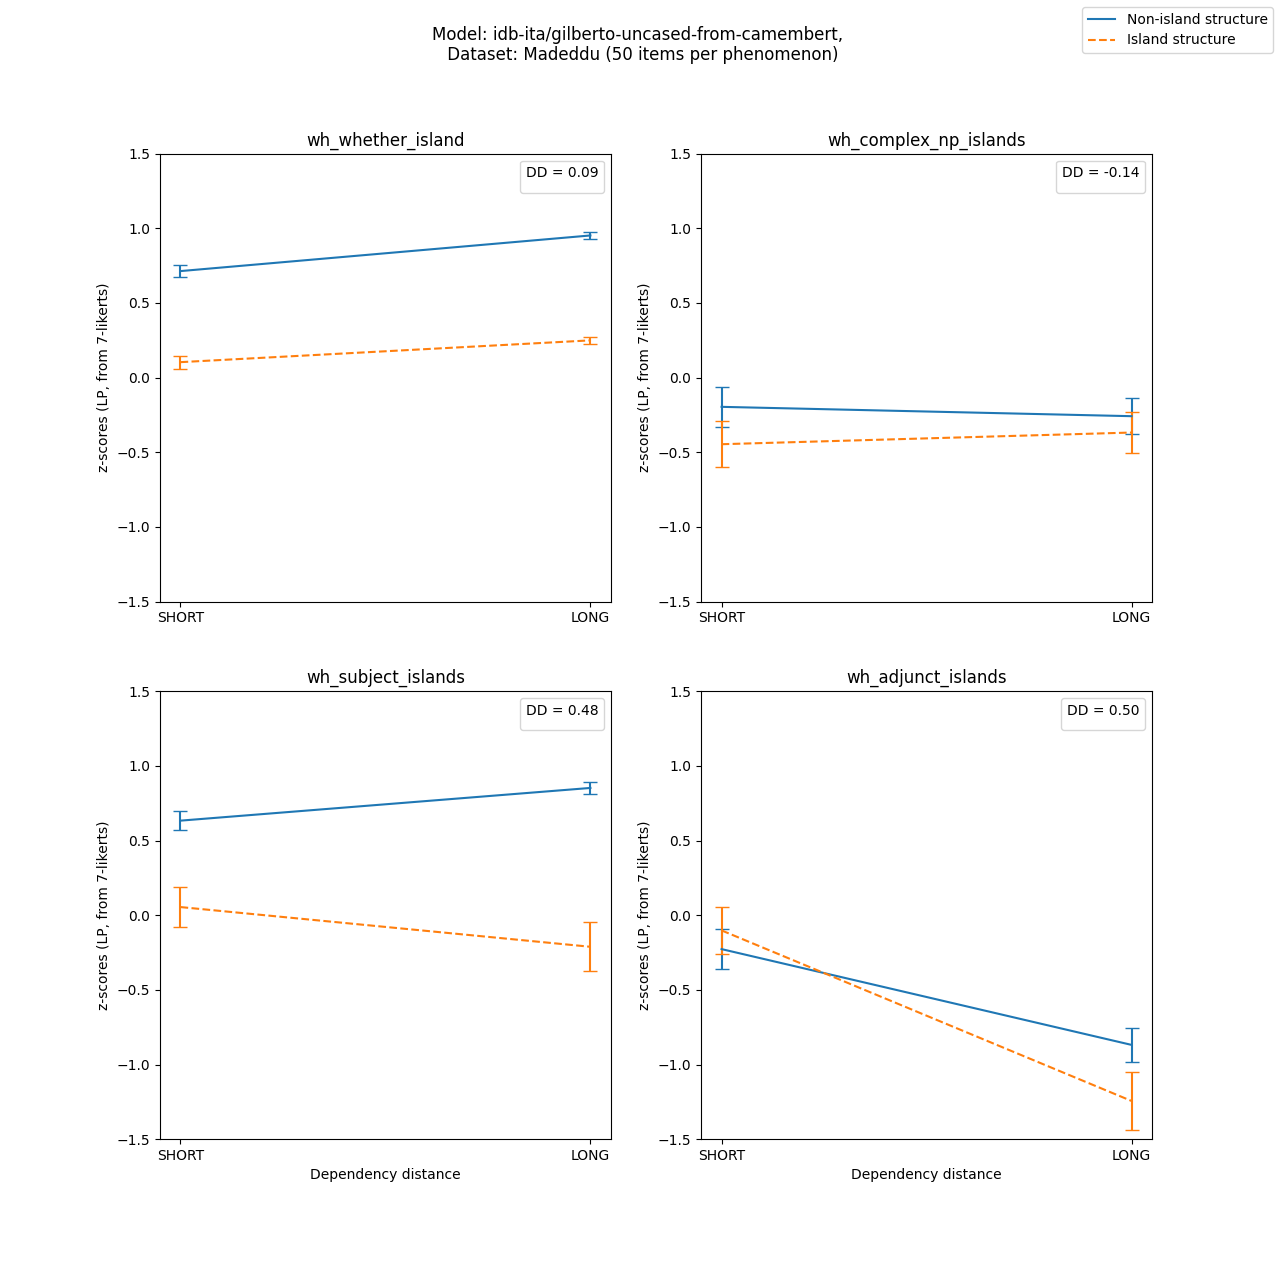
\includegraphics[width=1\textwidth]{images/AppendixA/Madeddu_wh_idb-ita_gilberto-uncased-from-camembert_LP-zscores-likert-2022-07-11.png} 
\end{figure}

\clearpage
\subsubsection{GilBERTo with PenLP-L (from logistic function model output)}
\begin{figure}[h]
	\centering
	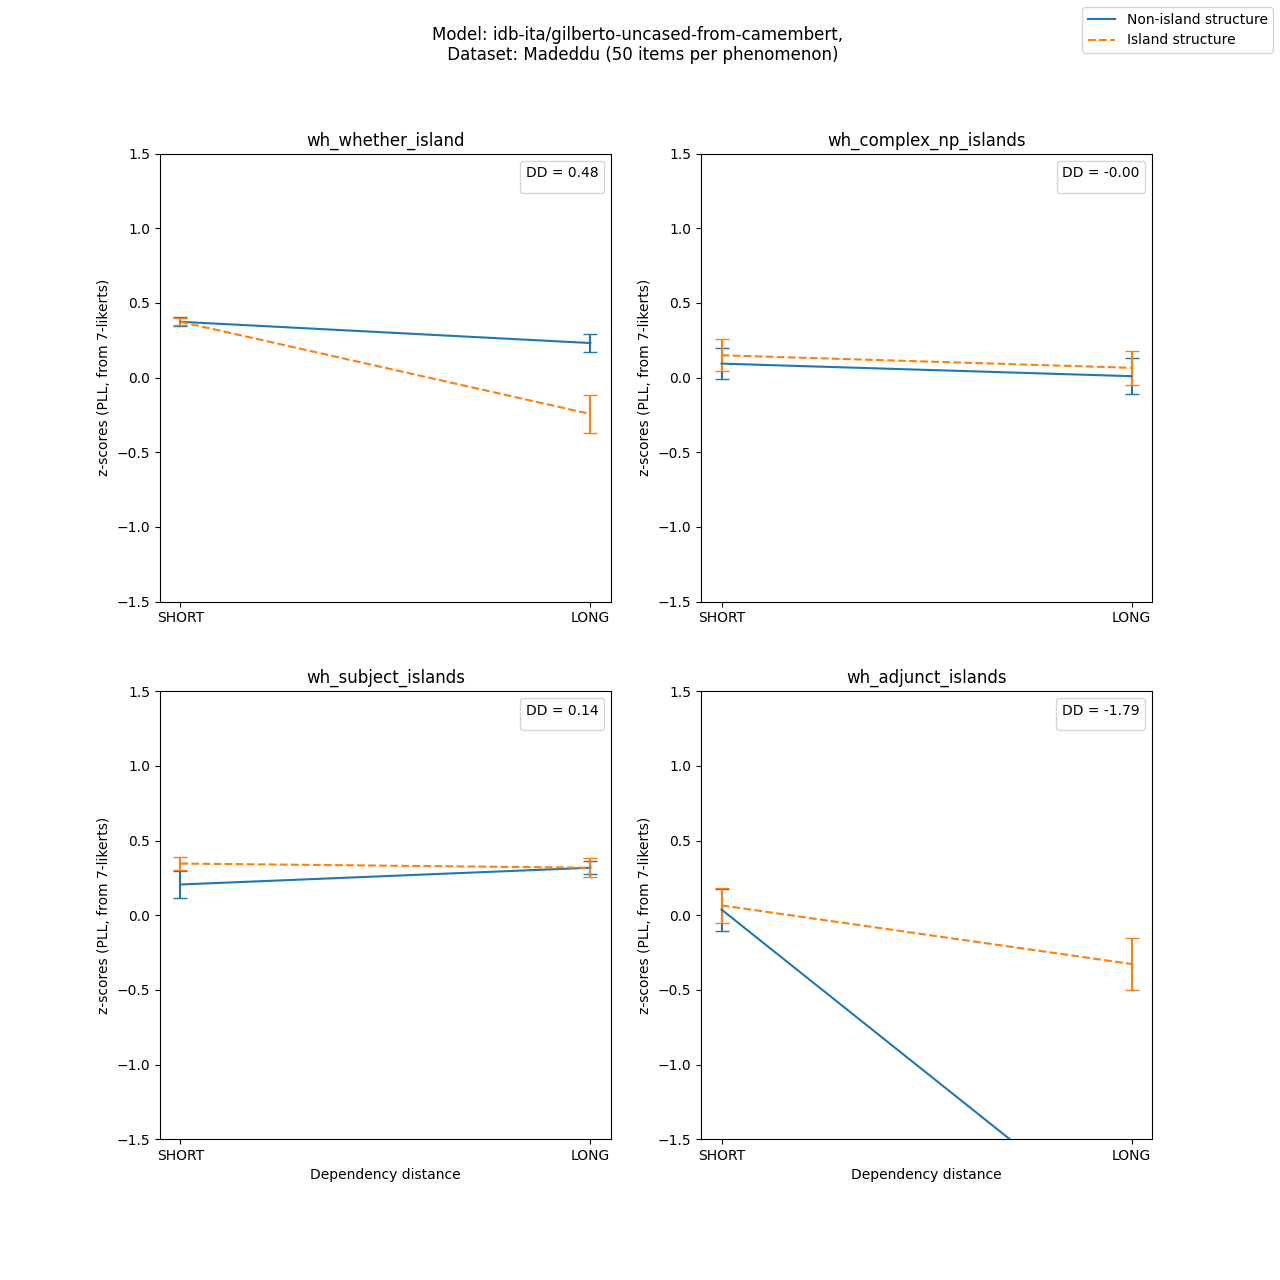
\includegraphics[width=1\textwidth]{images/AppendixA/Madeddu_wh_idb-ita_gilberto-uncased-from-camembert_PLL-zscores-likert-2022-07-11.png} 
\end{figure}

\clearpage
\subsubsection{GilBERTo with LP-L (from logistic function model output)}
\begin{figure}[h]
	\centering
	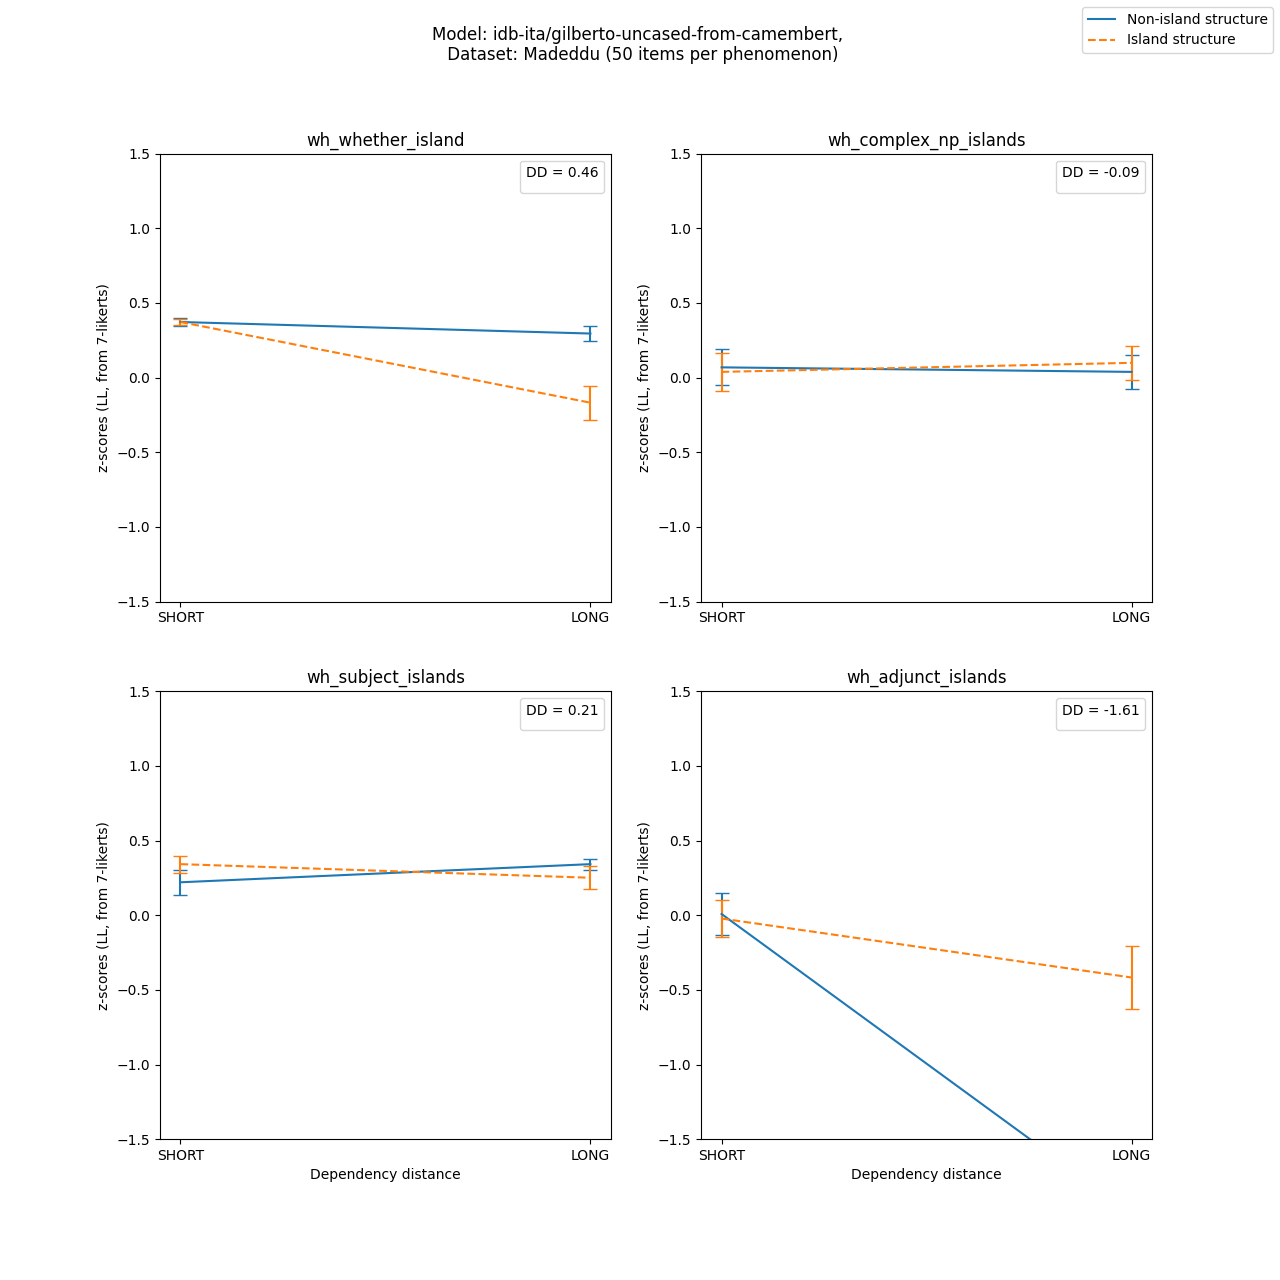
\includegraphics[width=1\textwidth]{images/AppendixA/Madeddu_wh_idb-ita_gilberto-uncased-from-camembert_LL-zscores-likert-2022-07-11.png} 
\end{figure}

\clearpage
\subsection{GePpeTto}

\subsubsection{GePpeTto with PenLP (from softmax model output)}
\begin{figure}[h]
	\centering
	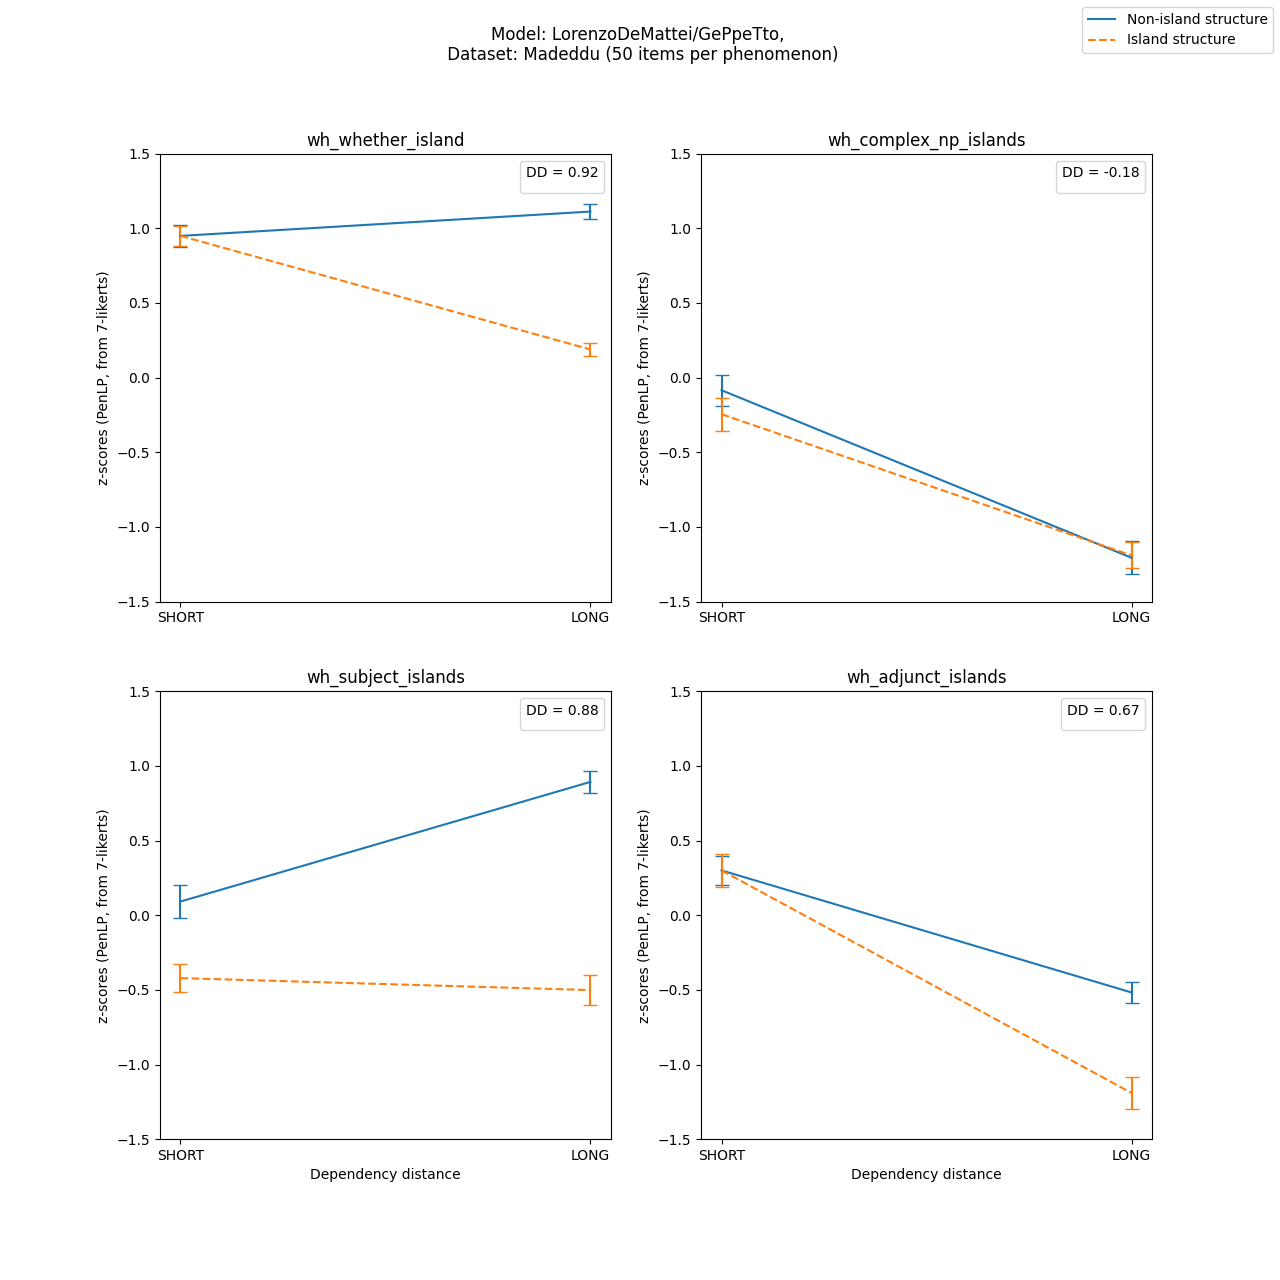
\includegraphics[width=1\textwidth]{images/AppendixA/Madeddu_wh_LorenzoDeMattei_GePpeTto_PenLP-zscores-likert-2022-07-11.png} 
\end{figure}

\clearpage
\subsubsection{GePpeTto with LP (from softmax model output)}
\begin{figure}[h]
	\centering
	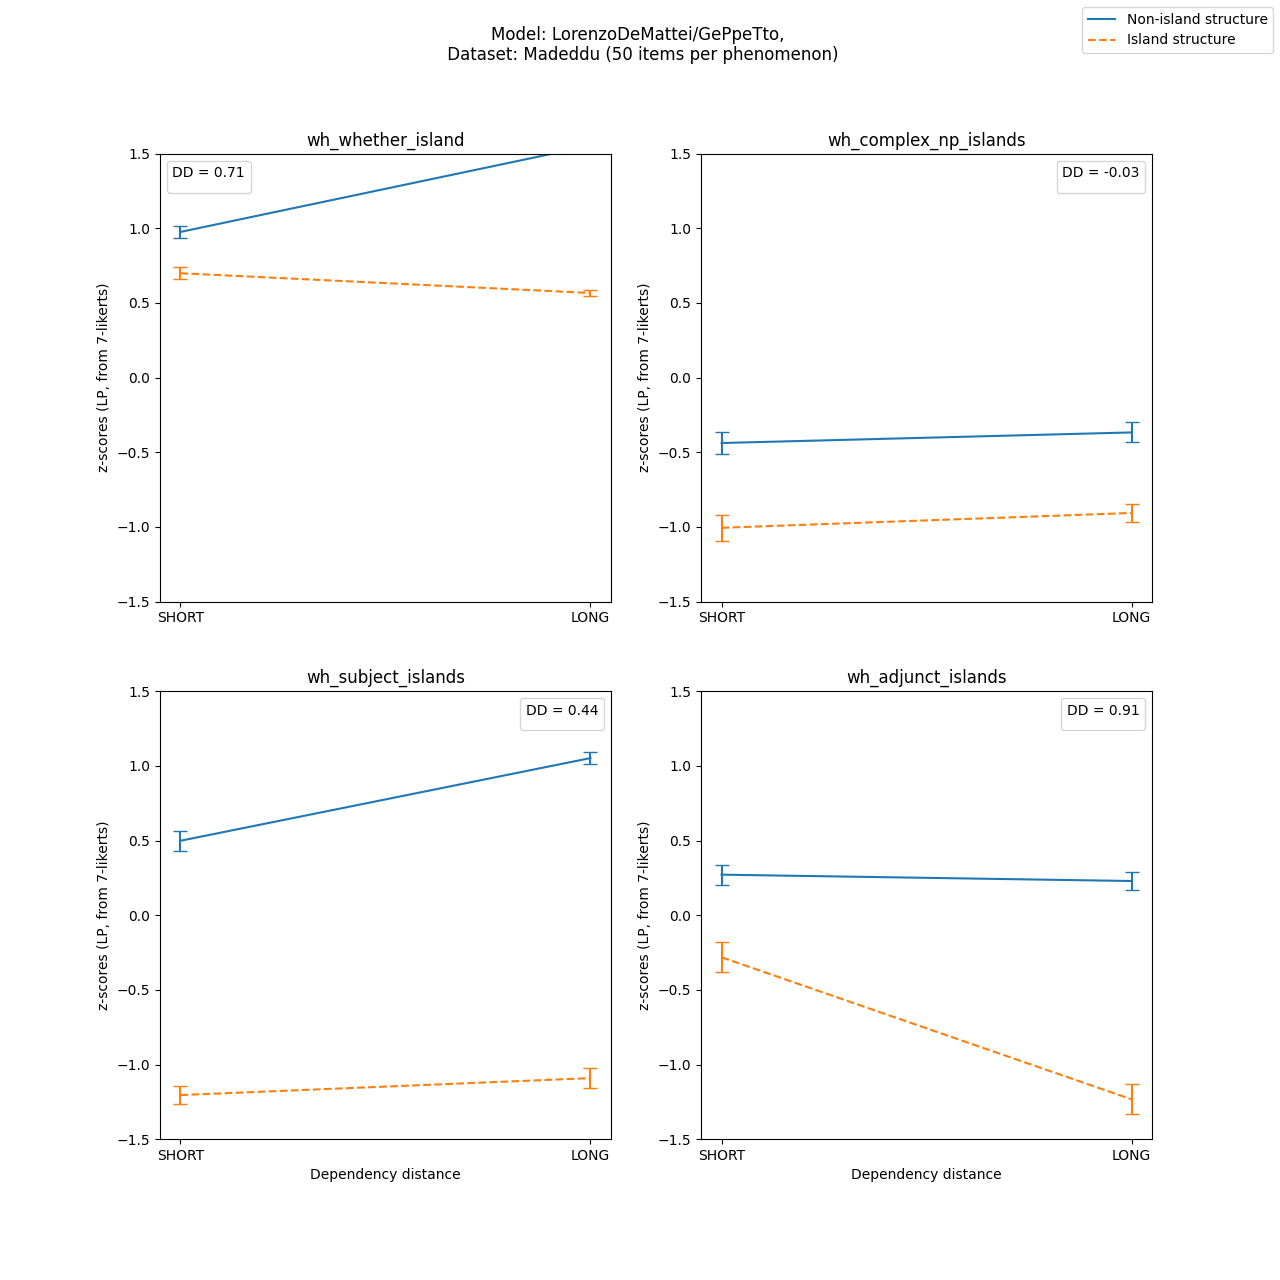
\includegraphics[width=1\textwidth]{images/AppendixA/Madeddu_wh_LorenzoDeMattei_GePpeTto_LP-zscores-likert-2022-07-11.png} 
\end{figure}




\bibliographystyle{agsm} 
\bibliography{chapters/Bibliography}


% .. 
% \addbibresource{references.bib}
% \include{chapters/Bibliografia}
\end{document}
% -----------------------------------------------------------------
